\renewcommand{\thechapter}{A}
\chapter{Appendix for Chapter~\ref{chap:ch1}}\label{APP:A}
% \phantomsection\addcontentsline{toc}{chapter}{Appendices}

\renewcommand{\thesection}{A.\arabic{section}}
\renewcommand{\thesubsection}{A.\arabic{section}.\arabic{subsection}}
\renewcommand{\thefigure}{A.\arabic{figure}}
\renewcommand{\thetable}{A.\arabic{table}}
\renewcommand{\theequation}{A.\arabic{equation}}

\section{Theoretical Proofs and Discussions}\label{App:proofs}
% \stoptoc

As mentioned in the main sections and Remark~\ref{ipm-remark}, most of our proofs hold even with a general IPM-regularized OT formulation (\ref{eqn:ipm-uot}) under mild assumptions. We restate such results and give a general proof that holds for IPM-regularized OT (Formulation~\ref{eqn:ipm-uot}), of which  MMD-regularized OT (Formulation~\ref{eqn:proposed}) is a special case. We first state the (mild) assumptions needed for the applicability of our proofs to the case of a general IPM-regularized OT. 

 Given a set $\calG\subset\calL(\calX)$, the integral probability metric (IPM)~\citep{mullergenset97,Sriperumbudur09onintegral,agrawal20a} associated with $\calG$, is defined by:
\begin{equation}\label{ipm-def}
     I_\calG(s_0,t_0)\equiv\max\limits_{f\in\calG}\left|\int_\calX f\ \textup{d}s_0-\int_\calX f\ \textup{d}t_0\right|\ \forall\ s_0,t_0\in\calR^+(\calX).
\end{equation}
$\calG$ is called the generating set of the IPM, $ I_\calG$.

\noindent In order that the IPM metrizes weak convergence, we assume the following~\citep{mullergenset97}:
\begin{assumption}\label{ass:genset1}
$\calG\subseteq\calC(\calX)$ and is compact.
\end{assumption}
\noindent Since the IPM generated by $\calG$ and its absolute convex hull is the same (without loss of generality), we additionally assume the following:
\begin{assumption}\label{ass:genset2}
$\calG$ is absolutely convex.
\end{assumption}
\begin{remark}
    We note that the assumptions 
\ref{ass:genset1} and~\ref{ass:genset2} are needed only to generalize our theoretical results to an IPM-regularized OT formulation (Formulation~\ref{eqn:ipm-uot}). These assumptions are satisfied whenever the IPM employed for regularization is the MMD (Formulation~\ref{eqn:proposed}) with a kernel that is continuous and universal (i.e., c-universal).
\end{remark}

\begin{definitionBoxIntro}
The proposed \textbf{IPM-regularized OT} formulation is presented as follows.
\begin{align}\label{eqn:ipm-uot}
\calWI(s_0, t_0)\coloneqq \min \limits_{\pi\in\calR^+\left(\calX\times\calX\right)} \int c ~\textup{d}\pi + \lambda_1  I_\calG(\pi_1, s_0) + \lambda_2  I_\calG(\pi_2,t_0),
\end{align}
where $ I_\calG$ is defined in \ref{ipm-def} and $\Lambda=\{\lambda_1, \ \lambda_2\}$.
\end{definitionBoxIntro}

We now present the theoretical results with IPM-regularized OT (Formulation~\ref{eqn:ipm-uot}), of which MMD-regularized OT (Formulation~\ref{eqn:proposed}) is a special case. To the best of our knowledge, such an analysis for IPM-regularized OT has not been done before.
\subsection[Deriving the Dual of MMD-OT]{Proof of Theorem~\ref{thm:dual}}\label{proof:thm-dual}
We state and prove the theorem with IPM-regularized OT formulation, for which the proof of Theorem~\ref{thm:dual} is a special case. This duality result leads us to several corollaries, restated and proved with the general IPM-regularized OT, of which MMD-OT is a special case.

For deriving the dual of the formulation with regularization based on a general IPM (other than MMD), we use the Assumptions~\ref{ass:genset1} and~\ref{ass:genset2} on the corresponding generating set.
\begin{remark}
Whenever the kernel, $k$, employed is continuous, the generating set of the corresponding MMD satisfies the Assumptions~\ref{ass:genset1} and~\ref{ass:genset2}. Hence, the duality proof of IPM-regularized OT (Theorem~\ref{app-thm:dual}) also works in the case of MMD-regularized OT  (i.e., to prove Theorem~\ref{thm:dual}).
\end{remark}
\begin{theoremBox}
\begin{theorem}[Dual of IPM-regularized OT]\label{app-thm:dual}
Whenever $\calG$ satisfies Assumptions~\ref{ass:genset1} and~\ref{ass:genset2}, $c\in\calC(\calX\times\calX)$, $\calX$ is compact and additionally kernel $k\in \calC(\calX\times\calX)$ for the case when the IPM is $\MMD_k$, we have the following.
\begin{align}\label{app:eqn-dual}
\calWI\left(s_0,t_0\right)=&\max\limits_{f\in\calG(\lambda_1),g\in\calG(\lambda_2)}\int_\calX f\ \textup{d}s_0+\int_\calX g\ \textup{d}t_0, \nonumber\\
&\ \ \ \ \ \ \ \ \ \textup{s.t.}\ \ \ \ \ \  f(x)+g(y)\le c(x,y)\ \forall\ x,y\in\calX.
\end{align}
\end{theorem}
\end{theoremBox}
\begin{proof}
We begin by re-writing the RHS of \ref{eqn:ipm-uot} using the definition of IPMs given in \ref{ipm-def}:
\allowdisplaybreaks
\begin{equation}\label{mmdual}
\begin{split}
\calWI\left(s_0,t_0\right)=&\min\limits_{\pi\in\calR^+\left(\calX\times\calX\right)}\  \int_{\calX\times\calX}c\ \textup{d}\pi + \lambda_1\left( \max\limits_{f\in\calG}\left|\int_\calX f\ \textup{d}s_0-\int_\calX f\ \textup{d}\pi_1\right|\right) \nonumber\\&\qquad\qquad\qquad\qquad\quad+ \lambda_2 \left(\max\limits_{g\in\calG}\left|\int_\calX g\ \textup{d}t_0-\int_\calX g\ \textup{d}\pi_2\right|\right)\\
\overset{\because (\ref{ass:genset2})}{=}&\min\limits_{\pi\in\calR^+\left(\calX\times\calX\right)}\  \int_{\calX\times\calX}c\ \textup{d}\pi + \lambda_1\left( \max\limits_{f\in\calG}\int_\calX f\ \textup{d}s_0-\int_\calX f\ \textup{d}\pi_1\right) \nonumber\\&\qquad\qquad\qquad\qquad\quad+ \lambda_2 \left(\max\limits_{g\in\calG}\int_\calX g\ \textup{d}t_0-\int_\calX g\ \textup{d}\pi_2\right)\\
=&\min\limits_{\pi\in\calR^+\left(\calX\times\calX\right)}\  \int_{\calX\times\calX}c\ \textup{d}\pi + \left( \max\limits_{f\in\calG(\lambda_1)}\int_\calX f\ \textup{d}s_0-\int_\calX f\ \textup{d}\pi_1\right) \nonumber\\&\qquad\qquad\qquad\qquad\quad~ +  \left(\max\limits_{g\in\calG(\lambda_2)}\int_\calX g\ \textup{d}t_0-\int_\calX g\ \textup{d}\pi_2\right)\\
=&\max\limits_{f\in\calG(\lambda_1),g\in\calG(\lambda_2)}\int_\calX f\ \textup{d}s_0+\int_\calX g\ \textup{d}t_0+\min\limits_{\pi\in\calR^+\left(\calX\times\calX\right)}\Bigg(\  \int_{\calX\times\calX}c\ \textup{d}\pi - \int_\calX f\ \textup{d}\pi_1 \\
& \qquad\qquad\qquad\qquad\qquad \qquad\qquad\qquad\qquad\qquad- \int_\calX g\ \textup{d}\pi_2\Bigg)\\
=&\max\limits_{f\in\calG(\lambda_1),g\in\calG(\lambda_2)}\int_\calX f\ \textup{d}s_0+\int_\calX g\ \textup{d}t_0+\min\limits_{\pi\in\calR^+\left(\calX\times\calX\right)}\  \int_{\calX\times\calX}c-\bar{f}-\bar{g}\ \textup{d}\pi\\
=&\max\limits_{f\in\calG(\lambda_1),g\in\calG(\lambda_2)}\int_\calX f\ \textup{d}s_0+\int_\calX g\ \textup{d}t_0+\left\{\begin{array}{cc}
    0 & \begin{array}{c}\textup{if } f(x)+g(y)\le c(x,y)\\ \forall\ x,y\in\calX,\end{array}\\
    -\infty & \textup{otherwise.}
    \end{array}\right.\\
    =&\max\limits_{f\in\calG(\lambda_1),g\in\calG(\lambda_2)}\int_\calX f\ \textup{d}s_0+\int_\calX g\ \textup{d}t_0,\\
    &\ \ \ \ \ \ \ \ \ \textup{s.t.}\ \ \ \ \ \  f(x)+g(y)\le c(x,y)\ \forall\ x,y\in\calX.
\end{split}    
\end{equation}
Here, $\bar{f}(x,y)\equiv f(x),\ \bar{g}(x,y)\equiv g(y)$. The min-max interchange in the third equation is due to Sion's minimax theorem: (i) since $\calR(\calX)$ is a topological dual of $\calC(\calX)$ whenever $\calX$ is compact, the objective is bilinear (inner-product in this duality), whenever $c,f,g$ are continuous. This is true from Assumption~\ref{ass:genset1} and $c\in\calC(\calX\times\calX)$. (ii) one of the feasibility sets involves $\calG$, which is convex compact by Assumptions~\ref{ass:genset1},~\ref{ass:genset2}. The other feasibility set is convex (the closed conic set of non-negative measures).
\end{proof}


\subsection[Proof of Metricity of MMD-OT]{Proof of Corollary~\ref{corr:ipm}}\label{proof:corr-metricity}
We first derive an equivalent reformulation of~\ref{eqn:ipm-uot}, which will be used in our proof.
\begin{lemmaBox}
\begin{lemma}\label{lemma:wipm-proposed}
\begin{equation}\label{eqn:proposedeq}
    \calWI\left(s_0,t_0\right) \equiv\min\limits_{s,t\in\calR^+(\calX)}\  |s| W_{c, 1}(s,t) + \lambda_1  I_\calG(s,s_0) + \lambda_2  I_\calG(t,t_0),
\end{equation}
where $W_{c, 1}(s,t)\equiv\left\{\begin{array}{cc}
    \bar{W}_{c,1}(\frac{s}{|s|},\frac{t}{|t|}) & \textup{ if } |s|=|t|, \\
    \infty & \textup{ otherwise}.
\end{array}\right.$, with $\bar{W}_{c,1}$ as the 1-Wasserstein metric.
\end{lemma}
\end{lemmaBox}
\begin{proof}
\begin{align}
    &\quad \min\limits_{s,t\in\calR^+(\calX)}\  |s| W_{c, 1}(s,t) + \lambda_1  I_\calG(s,s_0) + \lambda_2  I_\calG(t,t_0) \nonumber\\
    & = \min\limits_{s,t\in\calR^+(\calX);~|s|=|t|} |s| \min\limits_{\bar{\pi}\in \calR_1^+\left(\calX\times\calX\right)} \int c \ \textup{d}\bar{\pi} + \lambda_1  I_\calG(s, s_0)+\lambda_2  I_\calG(t, t_0) \ \textup{ s.t. }\bar{\pi}_1=\frac{s}{|s|}, \bar{\pi}_2=\frac{t}{|t|} \nonumber \\
    & = \min\limits_{\eta>0} ~ \eta \min\limits_{\bar{\pi}\in \calR_1^+\left(\calX\times\calX\right)} \int c \ \textup{d}\bar{\pi} + \lambda_1  I_\calG(\eta\bar{\pi}_1, s_0)+\lambda_2  I_\calG(\eta\bar{\pi}_2, t_0) \nonumber \\
    & = \min\limits_{\eta>0} ~ \min\limits_{\bar{\pi}\in \calR_1^+\left(\calX\times\calX\right)} \int c\ \eta \ \textup{d}\bar{\pi} +\lambda_1  I_\calG(\eta\bar{\pi}_1, s_0)+\lambda_2  I_\calG(\eta\bar{\pi}_2, t_0) \nonumber\\
    & = \min\limits_{\pi\in\calR^+\left(\calX\times \calX\right)}\int c ~\textup{d}\pi+\lambda_1  I_\calG(\pi_1, s_0)+\lambda_2  I_\calG(\pi_2, t_0) \nonumber
\end{align}
The first equality holds from the definition, $W_{c,1}(s,t)\equiv\left\{\begin{array}{cc}
    \bar{W}_{c, 1}(\frac{s}{|s|},\frac{t}{|t|}) & \textup{ if } |s|=|t|, \\
    \infty & \textup{ otherwise}.
\end{array}\right.$. Eliminating normalized versions $s$ and $t$ using the equality constraints and introducing $\eta$ to denote their common mass gives the second equality.  The last equality comes after changing the variable of optimization to $\pi\in\calR^+\left(\calX\times \calX\right) \equiv \eta\bar{\pi}$. Recall that $\calR^+(\calX)$ denotes the set of all non-negative Radon measures defined over $\calX$; while the set of all probability measures is denoted by $\calR^+_1(\calX)$.
\end{proof}

Corollary~\ref{corr:ipm} is restated below with the general IPM-regularized OT formulation (\ref{eqn:ipm-uot}), followed by its proof. The proof uses the equivalent reformulation presented in Lemma~\ref{lemma:wipm-proposed}. Our metricity proof needs $\lambda_1=\lambda_2$, and we will use the same for the subsequent proofs unless otherwise mentioned.
\begin{corollaryBox}
\begin{corollary}[Metricity of MMD-OT; generalized to IPM-regularized OT]\label{corr:ipm-duplicate}
In addition to assumptions in Theorem \ref{thm:dual}, whenever $c$ is a metric and $\lambda_1=\lambda_2=\lambda$, then we have the following.
\begin{itemize}
    \item $\calWI$ belongs to the family of integral probability metrics (IPMs).
    \item The generating set of this IPM is the intersection of the generating set of the Kantorovich metric, and the generating set of the IPM used for regularization.
    \item $\calWI$ is a valid norm-induced metric over measures whenever the IPM used for regularization is norm-induced (e.g. MMD with a characteristic kernel). Thus, $\calU$ \emph{lifts} the ground metric $c$ to that over measures.
\end{itemize} 
\end{corollary}
\end{corollaryBox}
\begin{proof}
The constraints in dual, (\ref{uot-eqn:dual}), are equivalent to: $g(y)\le\min\limits_{x\in\calX}c(x,y)-f(x)\ \forall\ y\in\calX$. The RHS is nothing but the $c$-conjugate ($c$-transform) of $f$. From \citet[Proposition~(6.1)]{peyre2019computational}, whenever $c$ is a metric we have the simplification, $\min\limits_{x\in\calX}c(x,y)-f(x)=\left\{\begin{array}{cc}
    -f(y) & \textup{if } f\in\calW_c,\\
    -\infty & \textup{otherwise}.
\end{array}\right.$ Here, $\calW_c$ is the generating set of the Kantorovich metric lifting $c$. Thus the constraints are equivalent to: $g(y)\le-f(y)\ \forall\ y\in\calX, f\in\calW_c$.
 
% By symmetry, we also obtain that $f(y)\le-g(y)\ \forall\ y\in\calX, g\in\calW_d$. 
Now, since the dual, (\ref{uot-eqn:dual}), seeks to maximize the objective with respect to $g$, and monotonically increases with values of $g$; at optimality, we have $g(y)=-f(y)\ \forall\ y\in\calX$. Note that this equality is possible to achieve as both $g,-f\in\calG(\lambda)\cap\calW_c$ (these sets are absolutely convex). Eliminating $g$, one obtains:
\begin{align}\label{app:eqn-dual1}
    \calWI\left(s_0,t_0\right)=&\max\limits_{f\in\calG(\lambda)\cap\calW_c}\int_\calX f\ \textup{d}s_0-\int_\calX f\ \textup{d}t_0,
\end{align}
    Comparing this and the definition of IPMs, we have that $\calWI$ belongs to the family of IPMs. Since any IPM is a pseudo-metric (induced by a semi-norm) over measures~\citep{mullergenset97}, the only condition left to be proved is positive definiteness with $\calWI(s_0, t_0)$. Following Lemma~\ref{lemma:wipm-proposed}, we have that for optimal $s^*,t^*$ in \ref{eqn:proposedeq}, 
    $\calWI(s_0, t_0)=0\iff (i)\ W_{c, 1}(s^*, t^*)=0, (ii)\  I_\calG(s^*, s_0)=0, (iii)\  I_\calG(t^*, t_0)=0$ as each term in the RHS is non-negative. When the IPM used for regularization is a norm-induced metric (e.g. the MMD metric or the Dudley metric), the conditions $(i), (ii), (iii)\iff s^*=t^*=s_0=t_0$, which proves the positive definiteness. Hence, we proved that $\calWI$ is a norm-induced metric over measures whenever the IPM used for regularization is a metric.
\end{proof}
\begin{remark}
    Recall that MMD is a valid norm-induced IPM metric whenever the kernel employed is characteristic. Hence, our proof above also shows the metricity of the MMD-regularized OT (as per Corollary~\ref{corr:ipm}).
\end{remark}
\begin{remark}
If $\calG$ is the unit uniform-norm ball (corresponding to TV), our result specializes to that in~\cite{pic2016}, which proves that $\calWI$ coincides with the so-called Flat metric (or the bounded Lipschitz distance).
\end{remark}
\begin{remark}
If the regularizer is the Kantorovich metric\footnote{The ground metric in $\calWI$ must be the same as that defining the Kantorovich regularizer.}, i.e., $\calG=\calW_c$, and $\lambda_1=\lambda_2=\lambda\ge1$, then the resulting divergence coincides with the Kantorovich metric. In other words, the Kantorovich-regularized OT is the same as the Kantorovich metric. Hence providing an OT interpretation for the Kantorovich metric that is valid for potentially unnormalized measures in $\calR^+(\calX)$.% So our result, in this case, can be viewed as  a generalization of the Kantorovich-Fenchel duality result.
\end{remark}

\subsection[Proof of MMD-OT Interpolating between Kantorovich and MMD]{Proof of Corollary~\ref{interp}}\label{proof:corr-interp}
\interpolant*
\begin{proof}
As discussed in Theorem~\ref{thm:dual} and Corollary~\ref{corr:ipm}, MMD-OT (Formulation~\ref{eqn:proposed}) results in an IPM with the generating set as an intersection of the generating sets of the MMD and the Kantorovich-Wasserstein metrics.
We now present special cases when MMD-OT (Formulation~\ref{eqn:proposed}) recovers back the Kantorovich-Wasserstein metric and the MMD metric.
\paragraph{Recovering Kantorovich.} Recall that $\calG_k(\lambda)=\{\lambda g~|~ g\in \calG_k\}$. From the definition of $\calG_k(\lambda)$, $f\in \calG_k(\lambda)\implies f\in \calH_k,~ \|f\|_k\leq \lambda$. Hence, as $\lambda\rightarrow \infty, \calG_k(\lambda)=\calH_k$. Using this in the duality result of Theorem~\ref{thm:dual}, we have the following.
\begin{align*}
\lim_{\lambda\rightarrow \infty}\calU(s_0, t_0)=\lim_{\lambda\rightarrow \infty}\max\limits_{f\in \calG_k(\lambda)\cap \calW_c}\int f \textup{d}s_0 - \int f \textup{d}t_0=&\max\limits_{f\in \calH_k\cap \calW_c}\int f \textup{d}s_0 - \int f \textup{d}t_0\\
\stackrel{(1)}{=}& \max\limits_{f\in \calC(\calX)\cap \calW_c}\int f \textup{d}s_0 - \int f \textup{d}t_0\\
\stackrel{(2)}{=}& \max\limits_{f\in \calW_c}\int f \textup{d}s_0 - \int f \textup{d}t_0
\end{align*}
Equality $(1)$ holds because $\calH_k$ is dense in the set of continuous functions, $\calC(\calX)$. For equality $(2)$, we use that $\calW_c$ consists of only 1-Lipschitz continuous functions. Thus, $\forall s_0, t_0\in \calR^+(\calX)$, $\lim_{\lambda\rightarrow\infty}\calU(s_0, t_0)=\calK_c(s_0, t_0).$ 

\paragraph{Recovering MMD.} We next show that when $0<\lambda_1=\lambda_2=\lambda\leq 1$ and the cost metric $c$ is such that 
\newline
$c(x, y)\geq \sqrt{k(x, x)+k(y, y)-2k(x, y)}=\|\phi_k(x)-\phi_k(y)\|_k~\forall x, y$ (Dominating Cost Assumption discussed in~\ref{dominating}), then $\forall s_0, t_0\in\calR^+(\calX)$,  $\calU(s_0, t_0)=\MMD_k(s_0, t_0)$.

Let $f\in \calG_k(\lambda)\implies f=\lambda g$ where $g\in \calH_k, \|g\|_k\leq 1$. This also implies that $\lambda g\in \calH_k$ as $\lambda\in(0,1]$.
\begin{align*}
    |f(x)-f(y)| &= |\left<\lambda g, \phi_k(x)-\phi_k(y) \right>| \tag{Reproducing property}\\
    &\leq |\left<g, \phi_k(x)-\phi_k(y) \right>| \ \tag{$\because 0<\lambda \leq 1$}\\
    &\leq \|g\|_k \|\phi_k(x)-\phi_k(y)\|_k \tag{Cauchy Schwarz}\\
    & \leq \|\phi_k(x)-\phi_k(y)\|_k \tag{$\because \|g\|\leq 1$}\\
    & \leq c(x, y) \tag{Dominating Cost Assumption}\\
    & \implies f\in \calW_c
\end{align*}
Therefore, $\calG_k(\lambda)\subseteq \calW_c$ and hence, $\calG_k(\lambda)\cap \calW_c = \calG_k(\lambda)$. This relation, together with the metricity result shown in Corollary~\ref{corr:ipm}, implies that $\calU(s_0, t_0)=\lambda \MMD_k(s_0, t_0)$. Next, in~\ref{dominating}, we show that the Euclidean distance satisfies the dominating cost assumption when the kernel employed is the Gaussian kernel and the inputs lie on a unit-norm ball.
\end{proof}
\subsection[Substantiating the Assumption on Cost Function to Recover MMD from MMD-OT]{Dominating Cost Assumption with Euclidean cost and Gaussian Kernel}\label{dominating} 
We present a sufficient condition for the Dominating Cost Assumption (used in Corollary~\ref{interp}) to be satisfied while using a Euclidean cost and an RBF kernel-based MMD.
We consider the characteristic RBF kernel, $k(x, y)=\exp{(-s\|x-y\|^2)}$, and show that for the hyperparameter, $0<s \leq 0.5$, the Euclidean cost is greater than the Kernel cost when the inputs are normalized, i.e., $\|x\|=\|y\|=1$.

\begin{align}\label{ineq}
    &\|x-y\|^2 \geq k(x, x) + k(y, y) - 2k(x, y) \\
    \iff &\|x\|^2 + \|y\|^2 - 2\left<x, y\right> \geq 2-2k(x, y) \nonumber\\
    \iff &\left<x, y\right> \leq \exp{\left(-2s(1-\left<x, y\right>)\right)} \tag{Assuming normalized inputs}
\end{align}
From Cauchy Schwarz inequality, $-\|x\|\|y\|\leq \left<x, y\right> \leq \|x\|\|y\|$. With the assumption of normalized inputs, we have that $-1\leq \left<x, y\right> \leq 1$. We consider two cases based on this.
\paragraph{Case 1: $\left<x, y\right>\in [-1, 0]$} In this case, condition \ref{ineq} is satisfied $\forall s\geq 0$ because $k(x, y)\geq 0 ~ \forall x, y$ with a Gaussian kernel.

\paragraph{Case 2: $\left<x, y\right>\in (0, 1]$} In this case, our problem in condition \ref{ineq} is to find $s\geq 0$ such that $\ln{\left<x, y\right>} \leq -2s(1-\left<x, y\right>)$. We further consider two sub-cases and derive the required condition as follows:
\paragraph{Case 2A: $\left<x, y\right>\in (0, \frac{1}{e}\big]$} We re-parameterize $\left<x, y\right> = e^{-n}$ for $n\geq 1$. With this, we need to find $s\geq 0$ such that $-n \leq -2s(1-e^{-n}) \iff n \geq 2s(1-e^{-n})$. This is satisfied when $0<s\leq 0.5$ because $e^{-n}\geq 1-n$.
\paragraph{Case 2B: $\left<x, y\right>\in (\frac{1}{e}, \infty)$} We re-parameterize $\left<x, y\right> = e^{-\frac{1}{n}}$ for $n> 1$. With this, we need to find $s\geq 0$ such that $\frac{1}{n\left(1-e^{-\frac{1}{n}}\right)} \geq 2s$. We consider the function $f(n)= n\left(1-e^{-\frac{1}{n}}\right)$ for $n\geq 1$. We now show that $f$ is an increasing function by showing that the gradient $\frac{\textup{d}f}{\textup{d}n} = 1-\left(1+\frac{1}{n} \right)e^{-\frac{1}{n}}$ is always non-negative.

\begin{equation*}
    \begin{split}
    &\frac{\textup{d}f}{\textup{d}n} \geq 0
    \\\iff & e^{\frac{1}{n}}  \geq \left( 1+ \frac{1}{n}\right)\\
    \iff & \frac{1}{n} - \ln{\left(1+ \frac{1}{n} \right)} \geq 0\\
    \iff & \frac{1}{n} - \left(\ln{(n+1)}-\ln{(n)}\right) \geq 0
    \end{split}
\end{equation*}
Applying the Mean Value Theorem on $g(n) = \ln{n}$, we get 
\begin{equation*}
    \begin{split}
        &\ln{(n+1)} - \ln{n} = (n+1-n)\frac{1}{z}, ~ \textup{where }n\leq z \leq n+1\\
        \implies & \ln{\left(1+ \frac{1}{n} \right)} = \frac{1}{z}\leq \frac{1}{n}\\
        \implies & \frac{\textup{d}f}{\textup{d}n} = \frac{1}{n} - \ln{\left(1+ \frac{1}{n} \right)} \geq 0
    \end{split}
\end{equation*}

The above shows that $f$ is an increasing function of $n$. We note that $\lim_{n\to \infty} f(n)=1$, hence, $\frac{1}{f(n)}=\frac{1}{n\left(1-e^{-\frac{1}{n}}\right)}\geq 1$ which implies that condition \ref{ineq} is satisfied by taking $0<s\leq 0.5$.

\subsection[Relation between MMD-OT, Kantorovich Metric and the involved IPM]{Proof of Corollary~\ref{corr:rel}}\label{proof:corr}
Corollary~\ref{corr:rel} is restated below with the general IPM-regularized OT formulation (\ref{eqn:ipm-uot}), followed by its proof.
\begin{corollaryBox}
\begin{corollary}[Relation between MMD-OT, Kantorovich Metric and MMD; generalized for IPM-regularized OT]
    $\calWI(s, t)\leq \min\left(\lambda I_\calG(s, t), \mathcal{K}_c(s, t)\right).$
\end{corollary}
\end{corollaryBox}
\begin{proof}
    Theorem~\ref{thm:dual} shows that $\calWI$ is an IPM whose generating set is the intersection of the generating sets of Kantorovich and the scaled version of the IPM used for regularization. Thus, from the definition of max, we have that $\calWI(s, t)\leq \lambda  I_\calG(s, t)$ and $\calWI(s, t)\leq \calK_c(s, t)$. This implies that $\calWI(s, t)\leq \min\left(\lambda I_\calG(s, t), \mathcal{K}_c(s, t)\right)$. As a special case, $\calU(s, t)\leq \min\left(\lambda\MMD_k(s, t), \calK_c(s, t)\right)$.
\end{proof}

\subsection[Proof of our Weak-Metrization Result]{Proof of Corollary~\ref{corr:weak}}\label{proof:corr-weak}
Corollary~\ref{corr:weak} is restated below with the general IPM-regularized OT formulation (\ref{eqn:ipm-uot}), followed by its proof.
\begin{corollaryBox}
\begin{corollary}[Weak Metrization; generalized for IPM-regularized OT]
    $\calWI$ metrizes the weak convergence of normalized measures.
\end{corollary}
\end{corollaryBox}
\begin{proof}
As $\calWI$ is a norm-induced metric, we have one side of the proof. We show the other side as follows. 
    From Corollary~\ref{corr:rel} proved above with the general IPM-regularized OT formulation,
    $0\leq \calWI(\beta_n, \beta) \leq \calK_c(\beta_n, \beta)$.
    \newline
    From Sandwich theorem, $\lim_{\beta_n\rightharpoonup \beta}\calWI(\beta_n, \beta)\rightarrow 0$ as $\lim_{\beta_n\rightharpoonup \beta}\calK_c(\beta_n, \beta) \rightarrow 0$.  From \citet[Theorem (6.9)]{villanioldnew}, we have that $\calK_c(\beta_n, \beta) \rightarrow 0$, which concludes the proof.
\end{proof}

\subsection[Proof of our Sample Complexity Result]{Proof of Corollary~\ref{corr:sampcomp}}\label{proof:corr-sc}
Corollary~\ref{corr:sampcomp} is restated below with the general IPM-regularized OT formulation (\ref{eqn:ipm-uot}), followed by its proof.
\begin{corollaryBox}
\begin{corollary}[Sample Complexity of IPM-regularized OT]
\label{app-corr:sampcomp}
Let $\hat{s}_m,\hat{t}_m$ denote the empirical estimates of $s_0,t_0 \in\calR^+(\calX)$ respectively with $m$ samples. Then, $\calWI(\hat{s}_m,\hat{t}_m)\rightarrow\calWI(s_0,t_0)$ at a rate (apart from constants)  same as that of $ I_\calG(\hat{s}_m,s_0)\rightarrow0$. 
\end{corollary}
\end{corollaryBox}
\begin{proof} 
    We use metricity of $\calWI$ proved in Corrolary~\ref{corr:ipm}. From triangle-inequality of the metric $\calWI$ and Corollary~\ref{corr:rel}, we have that
    \begin{align*}
    0\leq|\calWI(\hat{s}_m, \hat{t}_m)-\calWI(s_0, t_0)|&\leq \calWI(\hat{s}_m, s_0)+\calWI(t_0, \hat{t}_m)\\
    &\leq \lambda \left(I_\calG(\hat{s}_m, s_0)
    + I_\calG(\hat{t}_m, t_0)\right).
    \end{align*}
    
    Hence, by Sandwich theorem, $\calWI(\hat{s}_m, \hat{t}_m)\rightarrow \calWI(s_0, t_0)$ at a rate at which $ I_\calG(\hat{s}_m, s_0)\rightarrow 0$ and $ I_\calG(\hat{t}_m, t_0)\rightarrow 0$. If the IPM used for regularization is MMD with a normalized kernel, then $\MMD_k\left(s_0,\hat{s}_m\right)\le \sqrt{\frac{1}{m}}+\sqrt{\frac{2\log(1/\delta)}{m}}$ with probability at least $1-\delta$~\citep{SmolaGSS07}. From the union bound, with probability at least $1-\delta$, $$|\calU\left(\hat{s}_m,\hat{t}_m\right)-\calU\left(s_0,t_0\right)|\le 2\lambda\left(\sqrt{\frac{1}{m}}+\sqrt{\frac{2\log(2/\delta)}{m}}\right).$$
\end{proof}

\subsection[Proof of our Generalized Kantorovich Duality Result]{Proof of Theorem~\ref{thm:connkant}}\label{app:conn}
Before proving Theorem~\ref{thm:connkant}, we highlight that the result is not straightforward and is not a consequence of the Kantorovich-Rubinstein duality. This is because the regularization terms in our original formulation (\ref{eqn:ipm-uot}, \ref{eqn:proposedeq}) enforce closeness to the marginals of a transport plan and hence necessarily must be of the same mass and must belong to $\calR^+(\calX)$. Whereas in the RHS of \ref{eqn:ipmkant}, the regularization terms enforce closeness to marginals that belong to $\calR(\calX)$ and more importantly, they could be of different masses.

We restate the standard Moreau-Rockafellar theorem, which we refer to in our proof.
\begin{theorem}\label{thm:mr}
Let $X$ be a real Banach space and $f,g:X\mapsto\R\cup\{\infty\}$ be closed convex functions such that $dom(f)\cap dom(g)$ is not empty, then:
$(f+g)^*(y)=\min\limits_{x_1+x_2=y}f^*(x_1)+g^*(x_2)\ \forall y\in X^*$. Here, $f^*$ is the Fenchel conjugate of $f$, and $X^*$ is the topological dual space of $X$.
\end{theorem}

Theorem~\ref{thm:connkant} is restated below with the general IPM-regularized OT formulation~\ref{eqn:ipm-uot}, followed by its proof.
\begin{theoremBox}
\begin{theorem}[Generalized Kantorovich-Rubinstein Duality; generalized for IPM-regularized OT]
In addition to the assumptions in Theorem~\ref{thm:dual}, if $c$ is a valid metric, then
\begin{equation}\label{eqn:ipmkant}
    \calWI\left(s_0,t_0\right) =\min\limits_{s,t\in\calR(\calX)}\  \calK_c(s,t) + \lambda_1  I_\calG(s,s_0) + \lambda_2  I_\calG(t,t_0).
\end{equation}
 %the dual of the proposed IPM-regularized UOT, $\calWI\left(s_0,t_0\right)$, is the same as the dual of $\tilde{\calU}_{\calG,c,\lambda_1,\lambda_2}\left(s_0,t_0\right)$.
\end{theorem}\label{gen-kantdual}
\end{theoremBox}
\begin{proof}
We begin the proof by considering indicator functions $F_c$ and $F_\calG$ defined over $\calC(\calX)\times\calC(\calX)$ as: \newline
$F_c(f,g)=\Big\{\begin{array}{cc}
    0 & \textup{if } f(x)+g(y)\le c(x,y)\ \forall\ x,y\in\calX,\\
    \infty & \textup{otherwise}.
\end{array}$
, and 
\newline
$F_{\calG, \lambda_1, \lambda_2}(f,g)=\Big\{\begin{array}{cc}
    0 & \textup{if } f\in\calG(\lambda_1),g\in\calG(\lambda_2),\\
    \infty & \textup{otherwise.}
\end{array}$.

Recall that the topological dual of $\calC(\calX)$ is the set of regular Radon measures $\calR(\calX)$ and the duality product $\langle f,s\rangle\equiv\int f\  \textup{d}s\ \forall\ f\in\calC(\calX), s\in\calR(\calX)$. Now, from the definition of Fenchel conjugate in the (direct sum) space $\calC(\calX)\oplus\calC(\calX)$, we have: $$F_c^*(s,t)=\max\limits_{f\in\calC(\calX),g\in\calC(\calX)} \int f\ \textup{ds}+\int g\ \textup{dt}, \ \textup{s.t.} f(x)+g(y)\le c(x,y)\ \forall\ x,y\in\calX,$$ where $s,t\in\calR(\calX)$. Under the assumptions that $\calX$ is compact and $c$ is a continuous metric, \citet[Proposition~6.1]{peyre2019computational} shows that $$F_c^*(s,t)=\max\limits_{f\in\calW_c}\int f\textup{d} s - \int f\textup{d} t = \calK_c(s,t).$$ 

\noindent On the other hand, $$F_{\calG, \lambda_1, \lambda_2}(f,g)=\left(\max\limits_{f\in\calG(\lambda_1)} \int f\ \textup{ds} + \max\limits_{g\in\calG(\lambda_2)} \int g\ \textup{dt}\right)=\lambda_1 I_\calG(s,0)+\lambda_2 I_\calG(t,0).$$ Now, we have that the RHS of \ref{eqn:ipmkant} is $\min\limits_{s,t,s_1,t_1\in\calR(\calX):(s,t)+(s_1,t_1)=(s_0,t_0)}\ F^*_c(s,t)+F^*_{\calG, \lambda_1, \lambda_2}(s_1,t_1)$. This is because $ I_\calG(s_0-s,0)= I_\calG(s_0,s)$. Now, observe that the indicator functions $F_{\calG, \lambda_1, \lambda_2}, \ F_c$ are closed, convex functions because their domains are closed, convex sets. Indeed, $\calG$ is a closed, convex set by Assumptions~\ref{ass:genset1},\ \ref{ass:genset2}. Also, it is simple to verify that the set $\left\{(f,g)\ |\ f(x)+g(y)\le c(x,y)\ \forall\ x,y\in\calX\right\}$ is closed and convex. Hence, by applying the Moreau-Rockafellar formula (Theorem~\ref{thm:mr}), we have that the RHS of \ref{eqn:ipmkant} is equal to $\left(F_c + F_{\calG, \lambda_1, \lambda_2}\right)^*(s_0, t_0).$ But from the definition of conjugate, we have that $$\left(F_c + F_{\calG, \lambda_1, \lambda_2}\right)^*(s_0, t_0)\equiv\max\limits_{f\in\calC(\calX),g\in\calC(\calX)}\int_\calX f\ \textup{d}s_0+\int_\calX g\ \textup{d}t_0 - F_c(f,g) -F_{\calG, \lambda_1, \lambda_2}(f,g).$$ Finally, from the definition of the indicator functions $F_c$, $F_{\calG, \lambda_1, \lambda_2}$, this is same as the final RHS in \ref{mmdual}. Hence Proved.
\end{proof}
\begin{remark}
Whenever the kernel, $k$, employed is continuous, the generating set of the corresponding MMD satisfies assumptions~\ref{ass:genset1},\ \ref{ass:genset2} and $\calG_k\subseteq\calC(\calX)$. Hence, the above proof also works in our case of MMD-OT.
\end{remark}


\subsection[Proof of Consistency of the Proposed Estimator]{Proof of Theorem~\ref{thm:cons}}\label{cons}
\uotcons*
\begin{proof} 

From triangle-inequality, 
\begin{align}\label{inq:cons_ti}
|\hatcalUF(\hat{s}_m, \hat{t}_m)-\calU(s_0, t_0)| & \leq |\hatcalUF(\hat{s}_m, \hat{t}_m)-\hatcalUF(s_0, t_0)|\nonumber\\
&+|\hatcalUF(s_0, t_0)-\calU(s_0, t_0)|,
\end{align}
where $\hatcalUF(s_0, t_0)$ is same as $\calU(s_0, t_0)$ except that it employs the restricted feasibility set, $\calF(\hat{s}_m,\hat{t}_m)$, for the transport plan: set of all joints supported using the samples in $\hat{s}_m,\hat{t}_m$ alone i.e.,

$\calF(\hat{s}_m,\hat{t}_m)\equiv\left\{\sum_{i=1}^m\sum_{j=1}^m\bgamma_{ij}\delta_{(x_{1i},x_{2j})}\ |\ \bgamma_{ij}\ge0\ \forall\ i,j=1,\ldots,m\right\}$. Here, $\delta_z$ is the Dirac measure at $z$. We begin by bounding the first term in RHS of \ref{inq:cons_ti}.

We denote the (common) objective in $\hatcalUF(\cdot,\cdot),\ \calU(\cdot,\cdot)$ as a function of the transport plan, $\pi$, by $h(\pi,\cdot,\cdot)$. Then,
\allowdisplaybreaks
\begin{align*}
\hatcalUF(\hat{s}_m,\hat{t}_m)-\hatcalUF(s_0, t_0)&=\min\limits_{\pi\in \calF(\hat{s}_m,\hat{t}_m)}h(\pi,\hat{s}_m,\hat{t}_m)-\min\limits_{\pi\in \calF(\hat{s}_m,\hat{t}_m)}h(\pi,s_0,t_0)\nonumber\\
    &\le h(\pi^{0*}, \hat{s}_m, \hat{t}_m) - h(\pi^{0*}, s_0, t_0) \ \tag{where $\pi^{0*} = \argmin_{\pi\in \calF(\hat{s}_m,\hat{t}_m)}h(\pi,s_0,t_0)$}\nonumber\\
    &= \lambda_1 \left( \MMD_k(\pi^{0*}_1,\hat{s}_m) - \MMD_k(\pi^{0*}_1,s_0)\right) \\&\quad + \lambda_2\left( 
    \MMD_k(\pi^{0*}_2,\hat{t}_m) - \MMD_k(\pi^{0*}_2,t_0) \right)\nonumber \\
    & \le \lambda_1 \MMD_k(s_0,\hat{s}_m) + \lambda_2 \MMD_k(t_0,\hat{t}_m)\ \tag{$\because \MMD_k$ satisfies triangle-inequality} 
\end{align*}
Similarly, one can show that $\hatcalUF(s_0, t_0)-\hatcalUF(\hat{s}_m,\hat{t}_m)\leq \lambda_1 \MMD_k(s_0,\hat{s}_m) + \lambda_2 \MMD_k(t_0,\hat{t}_m)$. Now,~\citet[Theorem~3.4]{Muandet_2017} shows that, with probability at least $1-\delta$, $\MMD_k(s_0,\hat{s}_m)\le\frac{1}{\sqrt{m}}+\sqrt{\frac{2\log({1/\delta})}{m}}$, where $k$ is a normalized kernel. Hence, the first term in inequality \ref{inq:cons_ti} is upper-bounded by $(\lambda_1+\lambda_2)\left(\frac{1}{\sqrt{m}}+\sqrt{\frac{2\log{2/\delta}}{m}}\right)$, with probability at least $1-\delta$.

We next look at the second term in inequality \ref{inq:cons_ti}: $|\hatcalUF(s_0, t_0)-\calU(s_0, t_0)|$. Let $\bar{\pi}^m$ be the optimal transport plan in definition of $\hatcalUF(s_0, t_0)$. Let $\pi^*$ be the optimal transport plan in the definition of $\calU(s_0, t_0)$. Consider another transport plan: $\hat{\pi}^m\in \calF(\hat{s}_m,\hat{t}_m)$ such that $\hat{\pi}^m(x_i, y_j)=\frac{\eta(x_i, y_j)}{m^2}$ where $\eta(x_i, y_j)=\frac{\pi^*(x_i, y_j)}{s_0(x_i)t_0(y_j)}$ for $i, j\in [1,m]$. 
\begin{align*}
|\hatcalUF(s_0, t_0)-\calU(s_0, t_0)| &= \hatcalUF(s_0, t_0)-\calU(s_0, t_0)\\&= h(\bar{\pi}^m, s_0, t_0)-h(\pi^*, s_0, t_0)\\&\leq h(\hat{\pi}^m, s_0, t_0)-h(\pi^*, s_0, t_0)\ (\because \bar{\pi}^m \textup{ is optimal})\\
&\leq \int c~\textup{d}\hat{\pi}^m-\int c~\textup{d}\pi^*+\lambda_1 \|\mu_k(\hat{\pi}^m_1)-\mu_k(\pi^*_1)\|_k \\&\qquad\qquad\qquad\qquad\quad+ \lambda_2 \|\mu_k(\hat{\pi}^m_2)-\mu_k(\pi^*_2)\|_k \tag{from triangle-inequality.}
% & =\sum_{i=1}^m\sum_{j=1}^m c(x_i, y_j) \frac{\pi^*(x_i, y_j)}{m^2s_0(x_i)t_0(y_j)}-\int \int c(x, y) \frac{\pi^*(x, y)}{s_0(x)t_0(y)}s_0(x)t_0(y)~\textup{d}x~\textup{d}y\\&+\lambda_1 \|\mu_k(\hat{\pi}^m_1)-\mu_k(\pi^*_1)\|_k + \lambda_2 \|\mu_k(\hat{\pi}^m_2)-\mu_k(\pi^*_2)\|_k\\
% &=\E_{X\sim \hat{s}_m-s_0, Y\sim \hat{t}_m-t_0}\left[c(X, Y)\frac{\pi^*(X, Y)}{s_0(X)t_0(Y)}\right]+\lambda_1 \|\mu_k(\hat{\pi}^m_1)-\mu_k(\pi^*_1)\|_k + \lambda_2 \|\mu_k(\hat{\pi}^m_2)-\mu_k(\pi^*_2)\|_k\\
% &=\E_{X\sim \hat{s}_m-s_0, Y\sim \hat{t}_m-t_0}\left[c(X, Y)\eta(X,Y)\right]+\lambda_1 \|\mu_k(\hat{\pi}^m_1)-\mu_k(\pi^*_1)\|_k + \lambda_2 \|\mu_k(\hat{\pi}^m_2)-\mu_k(\pi^*_2)\|_k\\
\end{align*}

To upper bound these terms, we utilize the fact that the RKHS, $\calH_k$, corresponding to a c-universal kernel, $k$, is dense in $\calC(\calX)$ w.r.t. the sup-norm~\citep{SriperumbudurFL11} and like-wise the direct-product space, $\calH_k\otimes\calH_k$, is dense in $\calC(\calX\times\calX)$~\citep{gretton2015simpler}. Given any $f\in\calC(\calX)\times\calC(\calX)$, and arbitrarily small $\epsilon>0$, we denote by $f_\epsilon,f_{-\epsilon}$ the functions in $\calH_k\otimes\calH_k$ that satisfy the condition: $$f-\epsilon/2\le f_{-\epsilon}\le f\le f_\epsilon\le f+\epsilon/2.$$Such an $f_\epsilon\in\calH_k\otimes\calH_k$ will exist because: i) $f+\epsilon/4\in\calC(\calX)\times\calC(\calX)$ and ii) $\calH_k\otimes\calH_k\subseteq\calC(\calX)\times\calC(\calX)$ is dense. So there must exist some $f_\epsilon\in\calH_k\otimes\calH_k$ such that $|f(x,y)+\epsilon/4-f_\epsilon(x,y)|\le\epsilon/4\ \forall\ x,y\in\calX\iff f(x,y)\le f_\epsilon(x,y)\le f(x,y)+\epsilon/2\ \forall\ x,y\in\calX$. Analogously, $f_{-\epsilon}$ exists. In other words, $f_\epsilon,f_{-\epsilon}\in\calH_k\otimes\calH_k$ are arbitrarily close upper-bound (majorant), lower-bound (minorant) of $f\in\calC(\calX)\times\calC(\calX)$.

We now upper-bound the first of the set of terms (denote $s_0(x)t_0(y)$ by $\xi(x,y)$ and $\hatxi^m(x,y)$ is the corresponding empirical measure):
\begin{align*}
        \int c~\textup{d}\hat{\pi}^m-\int c~\textup{d}\pi^*&\le\int c_\epsilon~\textup{d}\hatpi^m-\int c_{-\epsilon}~\textup{d}\pi^*\\
        &=\langle c_\epsilon,\mu_k(\hatpi^m)\rangle-\langle c_{-\epsilon},\mu_k(\pi^*)\rangle\\
        &=\langle c_\epsilon,\mu_k(\hatpi^m)\rangle-\langle c_\epsilon,\mu_k(\pi^*)\rangle+\langle c_\epsilon,\mu_k(\pi^*)\rangle-\langle c_{-\epsilon},\mu_k(\pi^*)\rangle\\
        &=\langle c_\epsilon,\mu_k(\hatpi^m)-\mu_k(\pi^*)\rangle+\langle c_\epsilon-c_{-\epsilon},\mu_k(\pi^*)\rangle\\
        &\le \langle c_\epsilon,\mu_k(\hatpi^m)-\mu_k(\pi^*)\rangle + \epsilon\sigma_{\pi^*}\\
        &\tag{$\because \|c_\epsilon-c_{-\epsilon}\|_\infty\le\epsilon$ and $\sigma_{s}$ defined as the mass of measure $s$}\\
    & \le\|c_\epsilon\|_k\|\mu_k(\hatpi^m)-\mu_k(\pi^*)\|_k + \epsilon\sigma_{\pi^*}
\end{align*}
One can obtain the tightest upper bound by choosing $c_\epsilon\equiv\argmin_{v\in\calH_k\otimes\calH_k}\|v\|_k\ \ \textup{s.t.}\ c\le v\le c+\epsilon/2$. Accordingly, we replace $\|c\|_k$ by $g(\epsilon)$ in the theorem statement\footnote{This leads to a slightly weaker bound, but we prefer it for ease of presentation}.
Further, we have:
\allowdisplaybreaks
\begin{align*}
    \left\|\mu_k(\hat{\pi}^m)-\mu_k(\pi^*)\right\|_k^2
    &=\left\|\int\phi_k(x)\otimes\phi_k(y)\textup{d}\hat{\pi}^m(x,y)-\int\phi_k(x)\otimes\phi_k(y)\textup{d}\pi^*(x,y)\right\|_k^2\\
    &=\left\|\int\phi_k(x)\otimes\phi_k(y)\textup{d}\left(\hat{\pi}^m(x,y)-\pi^*(x,y)\right)\right\|_k^2\\
    &=\Bigg<\int\phi_k(x)\otimes\phi_k(y)\textup{d}\left(\hat{\pi}^m(x,y)-\pi^*(x,y)\right),\\
    &\quad\int\phi_k(x')\otimes\phi_k(y')\textup{d}\left(\hat{\pi}^m(x',y')-\pi^*(x',y')\right)\Bigg>\\
    &=\Bigg<\int\phi_k(x)\otimes\phi_k(y)\eta(x,y)\textup{d}\left(\hatxi^m(x,y)-\xi(x,y)\right),\\
    &\quad\int\phi_k(x')\otimes\phi_k(y')\eta(x',y')\textup{d}\left(\hatxi^m(x',y')-\xi(x',y')\right)\Bigg>\\
    &=\int\int\langle\phi_k(x)\otimes\phi_k(y),\phi_k(x')\otimes\phi_k(y')\rangle\eta(x,y)\eta(x',y')\\
    &\qquad\textup{d}\left(\hatxi^m(x,y)-\xi(x,y)\right)\ \textup{d}\left(\hatxi^m(x',y')-\xi(x',y')\right)\\
    &=\int\int\langle\phi_k(x),\phi_k(x')\rangle\langle\phi_k(y),\phi_k(y')\rangle\eta(x,y)\eta(x',y')\\
    &\qquad\qquad\textup{d}\left(\hatxi^m(x,y)-\xi(x,y)\right)\ \textup{d}\left(\hatxi^m(x',y')-\xi(x',y')\right)\\
    &=\int\int k(x,x')k(y,y')\eta(x,y)\eta(x',y')\textup{d}\left(\hatxi^m(x,y)-\xi(x,y)\right)\ \\
    &\qquad\qquad\qquad\qquad\qquad\qquad\qquad\quad\textup{d}\left(\hatxi^m(x',y')-\xi(x',y')\right).
\end{align*}
Now, observe that $\tilde{k}:\calX\times\calX\times\calX\times\calX$ defined by the product kernel $\tilde{k}\left((x,y),(x',y')\right)\equiv k(x,x')k(y,y')\eta(x,y)\eta(x',y')$ is a valid kernel. This is because $\tilde{k}=k_ak_bk_c$, where $k_a\left((x,y),(x',y')\right)\equiv k(x, x')$ is a kernel, $k_b\left((x,y),(x',y')\right)\equiv k(y, y')$ is a kernel, and $k_c\left((x,y),(x',y')\right)\equiv\eta(x,y)\eta(x',y')$ is a kernel (the unit-rank kernel), and product of kernels is indeed a kernel. Let $\psi(x,y)$ be the feature map corresponding to $\tilde{k}$. Then, the final RHS in the above set of equations is:
\begin{align*}
&=\int\int \langle\psi(x,y),\psi(x',y')\rangle\textup{d}\left(\hatxi^m(x,y)-\xi(x,y)\right)\ \textup{d}\left(\hatxi^m(x',y')-\xi(x',y')\right)\\
&=\left\langle\int\psi(x,y)\textup{d}\left(\hatxi^m(x,y)-\xi(x,y)\right),\int\psi(x',y')\textup{d}\left(\hatxi^m(x',y')-\xi(x',y')\right)\right\rangle. 
\end{align*}
Hence, we have that: $\left\|\mu_k(\hat{\pi}^m)-\mu_k(\pi^*)\right\|_k=\left\|\mu_{\tilde{k}}(\hatxi^m)-\mu_{\tilde{k}}(\xi)\right\|_{\tilde{k}}$. Again, using~\citet[Theorem~3.4]{Muandet_2017}, with probability at least $1-\delta$, $\left\|\mu_{\tilde{k}}(\hatxi^m)-\mu_{\tilde{k}}(\xi)\right\|_{\tilde{k}}\le\frac{C_{\tilde{k}}}{{m}}+\frac{\sqrt{2C_{\tilde{k}}\log({1/\delta})}}{m}$, where $C_{\tilde{k}}=\max\limits_{x,y,x',y'\in\calX}\tilde{k}\left((x,y),(x',y')\right)$. Note that $C_{\tilde{k}}<\infty$ as $\calX$ is compact and $s_0,t_0$ are assumed to be positive measures and $k$ is normalized.

Now the MMD-regularizer terms can be bounded using a similar strategy. Recall that, $\hat{\pi}^m_1(x_i)=\sum_{j=1}^n\frac{\pi^*(x_i, y_j)}{m^2s_0(x_i)t_0(y_j)}$, so we have the following.
\begin{align*}
    \left\|\mu_k(\hat{\pi}^m_1)-\mu_k(\pi^*_1)\right\|_k^2
    &=\left\|\int\phi_k(x)\textup{d}\hat{\pi}^m_1(x)-\int\phi_k(x)\textup{d}\pi^*_1(x)\right\|_k^2\\
    &=\left\|\int\phi_k(x)\textup{d}\left(\hat{\pi}^m_1(x)-\pi^*_1(x)\right)\right\|_k^2\\
    &=\left\langle\int\phi_k(x)\textup{d}\left(\hat{\pi}^m_1(x)-\pi^*_1(x)\right),\int\phi_k(x')\textup{d}\left(\hat{\pi}^m_1(x')-\pi^*_1(x')\right)\right\rangle\\
    &=\Bigg<\int\phi_k(x)\eta(x,y)\textup{d}\left(\hatxi^m(x,y)-\xi(x,y)\right),\\
    &\qquad\qquad \int\phi_k(x')\eta(x',y')\textup{d}\left(\hatxi^m(x',y')-\xi(x',y')\right)\Bigg>\\
    &=\int\int\langle\phi_k(x),\phi_k(x')\rangle\eta(x,y)\eta(x',y')\textup{d}\left(\hatxi^m(x,y)-\xi(x,y)\right)
    \\
    &\qquad\qquad\qquad\qquad\qquad\qquad\qquad\quad \textup{d}\left(\hatxi^m(x',y')-\xi(x',y')\right)\\
    &=\int\int k(x,x')\eta(x,y)\eta(x',y')\textup{d}\left(\hatxi^m(x,y)-\xi(x,y)\right)\\
    &\qquad\qquad\qquad\qquad\qquad\qquad \textup{d}\left(\hatxi^m(x',y')-\xi(x',y')\right).
\end{align*}
Now, observe that $\bark:\calX\times\calX\times\calX\times\calX$ defined by the product kernel, $\bark\left((x,y),(x',y')\right)\equiv k(x,x')\eta(x,y)\eta(x',y')$ is a valid kernel as $\bark=k_1k_2$, where $k_1\left((x,y),(x',y')\right)\equiv k(x, x')$ is a kernel and $k_2\left((x,y),(x',y')\right)\equiv\eta(x,y)\eta(x',y')$ is a kernel (the unit-rank kernel), and product of kernels is indeed a kernel. 

Hence, we have that: $\left\|\mu_k(\hat{\pi}^m_1)-\mu_k(\pi^*_1)\right\|_k=\left\|\mu_{\bark}(\hatxi^m)-\mu_{\bark}(\xi)\right\|_{\bark}$. Similarly, we have: $\left\|\mu_k(\hat{\pi}^m_2)-\mu_k(\pi^*_2)\right\|_k=\left\|\mu_{\bark}(\hatxi^m)-\mu_{\bark}(\xi)\right\|_{\bark}$.  Again, using~\citet[Theorem~3.4]{Muandet_2017}, with probability at least $1-\delta$, $\left\|\mu_{\bark}(\hatxi^m)-\mu_{\bark}(\xi)\right\|_{\bark}\le\frac{C_{\bark}}{{m}}+\frac{\sqrt{2C_{\bark}\log({1/\delta})}}{m}$, where $C_{\bark}=\max\limits_{x,y,x',y'\in\calX}\bark\left((x,y),(x',y')\right)$. Note that $C_{\bark}<\infty$ as $\calX$ is compact, $s_0,t_0$ are assumed to be positive measures, and $k$ is normalized.
From the union bound, $\left|\hatcalUF(\hat{s}_m, \hat{t}_m)-\calU(s_0, t_0)\right|\leq \left(\lambda_1+\lambda_2\right)\left(\frac{1}{\sqrt{m}}+\sqrt{\frac{2\log{(5/\delta)}}{m}}+\frac{C_{\bark}}{{m}}+\frac{\sqrt{2C_{\bark}\log({5/\delta})}}{m}\right)+g(\epsilon)\left(\frac{C_{\tilde{k}}}{{m}}+{\frac{\sqrt{2C_{\tilde{k}}\log{(5/\delta)}}}{m}}\right)+\epsilon\sigma_{\pi^*}$, with probability at least $1-\delta$. In other words, w.h.p. we have: $$\left|\hatcalUF(\hat{s}_m, \hat{t}_m)-\calU(s_0, t_0)\right|\leq O\left(\frac{\lambda_1+\lambda_2}{\sqrt{m}}+\frac{g(\epsilon)}{m}+\epsilon\sigma_{\pi^*}\right),$$ for any $\epsilon>0.$
\end{proof}
%%%


\subsubsection{Bounding $g(\epsilon)$}\label{app:bharath}
Let the target function to be approximated be $h^*\in\calC(\calX)\subset\calL^2(\calX)$, which is the set of square-integrable functions (w.r.t. some measure). Since $\calX$ is compact, $k$ being c-universal, it is also $\calL^2$-universal.

Consider the inclusion map $\iota:\calH_k\mapsto\calL^2(\calX)$, defined by $\iota\ g=g$. Let's denote the adjoint of $\iota$ by $\iota^*$. Consider the regularized least square approximation of $h^*$ defined by $h_t\equiv(\iota^*\iota+t)^{-1}\iota^*h^*\in\calH_k$, where $t>0$. Now, using standard results, we have:
\begin{align*}
    \|\iota h_t-h^*\|_{\calL^2}&=\|\left(\iota(\iota^*\iota+t)^{-1}\iota^*-I\right)h^*\|_{\calL^2}\\
    &=\|\left(\iota\ \iota^*(\iota\ \iota^*+t)^{-1}-I\right)h^*\|_{\calL^2}\\
    &=\|\left(\iota\ \iota^*(\iota\ \iota^*+t)^{-1}-(\iota\ \iota^*+t)(\iota\ \iota^*+t)^{-1}\right)h^*\|_{\calL^2}\\
    &=t\|\left(\iota\ \iota^*+t\right)^{-1}h^*\|_{\calL^2}\\
    &\le t\|\left(\iota\ \iota^*\right)^{-1}h^*\|_{\calL^2}\\
\end{align*}
The last inequality is true because the operator $\iota\ \iota^*$ is PD and $t>0$. Thus, if $t\equiv \hat{t}=\frac{\epsilon}{\|\left(\iota\ \iota^*\right)^{-1}h^*\|_{\calL^2}}$, then $\|\iota h_{\hat{t}} -h^*\|_\infty\le\|\iota h_{\hat{t}}-h^*\|_{\calL^2}\le\epsilon$. Clearly, 
\allowdisplaybreaks
\begin{align*}
 g(\epsilon)&\le\|h_{\hat{t}}\|_{\calH_k}\\
 &=\sqrt{\langle h_{\hat{t}},h_{\hat{t}}\rangle_{\calH_k}}\\
 &=\sqrt{\langle (\iota^*\iota+\hat{t})^{-1}\iota^*h^*,(\iota^*\iota+\hat{t})^{-1}\iota^*h^*\rangle_{\calH_k}}\\
 &=\sqrt{\langle \iota^*(\iota\ \iota^*+\hat{t})^{-1}h^*,\iota^*(\iota\ \iota^*+\hat{t})^{-1}h^*\rangle_{\calH_k}}\\
 &=\sqrt{\langle (\iota\ \iota^*+\hat{t})^{-1}\iota\ \iota^*(\iota\ \iota^*+\hat{t})^{-1}h^*,h^*\rangle_{\calL^2}}\\
 &=\sqrt{\langle \left(\iota\ \iota^*\right)^\frac{1}{2}(\iota\ \iota^*+\hat{t})^{-1}h^*,\left(\iota\ \iota^*\right)^\frac{1}{2}(\iota\ \iota^*+\hat{t})^{-1}h^*\rangle_{\calL^2}}\\
 &=\|\left(\iota\ \iota^*\right)^\frac{1}{2}(\iota\ \iota^*+\hat{t})^{-1}h^*\|_{\calL^2}.
\end{align*}
Now, consider the spectral function $f(\lambda)=\frac{\lambda^\frac{1}{2}}{\lambda+\hat{t}}$. This is maximized when $\lambda=\hat{t}$. Hence, $f(\lambda)\le\frac{1}{2\sqrt{\hat{t}}}$. Thus, $g(\epsilon)\le\frac{\|h^*\|_{\calL^2}\sqrt{\|\left(\iota\ \iota^*\right)^{-1}h^*\|_{\calL^2}}}{2\sqrt{\epsilon}}$. Therefore, as $\epsilon$ decays as $\frac{1}{m^{2/3}}$, then, $\frac{g(\epsilon)}{m}\le O\left(\frac{1}{m^{2/3}}\right)$.

% \subsection{Solving Problem (\ref{eqn:kernotinit}) using Mirror Descent}\label{appendix:md}
% Problem (\ref{eqn:kernotinit}) is an instance of a convex program and can be solved using Mirror Descent~\citep{Ne05}, presented in Algorithm~\ref{alg:md}.
% \begin{algorithm}
% \caption{Mirror Descent for solving Problem (\ref{eqn:kernotinit})}\label{alg:md}
% \begin{algorithmic}
% \Require Initial $\bgamma_1\geq 0$, max iterations $N$.
% \State $f(\bgamma) = \Tr\left(\bgamma\bC^\top\right) + \lambda_1\left\Vert\bgamma\bone-\frac{\sigma_1}{m}\bone\right\Vert_{\bG_{11}}+\lambda_2\left\Vert\bgamma^\top\bone-\frac{\sigma_2}{m}\bone\right\Vert_{\bG_{22}}$.
% \For{$i \gets 1$ to $N$}
% \If{$\|\nabla f(\bgamma_i)\|\neq \mathbf{0}$}
% \State $s_i = 1/\|\nabla f(\bgamma_i)\|_\infty$.
% \Else
% \State \textbf{return} $\bgamma_i$.
% \EndIf
% \State $\bgamma_{i+1} = \bgamma_{i}\odot e^{-s_i\nabla f(\bgamma_i)}$.
% \EndFor
% \end{algorithmic}
% \Return $\bgamma_{i+1}$.
% \end{algorithm}

\subsection[Equivalence between our OT Formulations with MMD and squared-MMD Regularizations]{Equivalence between Problems \ref{eqn:kernotinit} and \ref{eqn:kernot}}\label{Ivanov}
We comment on the equivalence between Problems \ref{eqn:kernotinit} and \ref{eqn:kernot} based on the equivalence of their Ivanov forms:

Ivanov form for Problem \ref{eqn:kernotinit} is
\begin{equation*}
    \min\limits_{\bgamma\ge \bzero} \Tr\left( \bgamma \bC^\top\right) \textup{ s.t. } \left\Vert\bgamma\bone-\frac{\sigma_1}{m_1}\bone\right\Vert_{\bG_{11}}\leq r_1, \left\Vert\bgamma^\top\bone-\frac{\sigma_2}{m_2}\bone\right\Vert_{\bG_{22}}\leq r_2, 
\end{equation*}
where $r_1, r_2>0$.

Similarly, the Ivanov form for Problem \ref{eqn:kernot} is
\begin{equation*}
    \min\limits_{\bgamma\ge \bzero} \Tr\left( \bgamma \bC^\top\right) \textup{ s.t. } \left\Vert\bgamma\bone-\frac{\sigma_1}{m_1}\bone\right\Vert^2_{\bG_{11}}\leq \bar{r}_1, \left\Vert\bgamma^\top\bone-\frac{\sigma_2}{m_2}\bone\right\Vert^2_{\bG_{22}}\leq \bar{r}_2,
\end{equation*}
where $\bar{r}_1, \bar{r}_2>0$.

As we can see, the Ivanov forms are the same with $\bar{r}_1=r_1^2, \bar{r}_2=r_2^2$, the solutions obtained for Problems (\ref{eqn:kernotinit}) and (\ref{eqn:kernot}) are the same.


\subsection[Deriving Step-Size for APGD-based Algorithm]{Proof of Lemma~\ref{apgd-L}}\label{proof:lemma-solve} 
\Lderiv*
\begin{proof}
Let $f(\bgamma)$ denote the objective of Problem \ref{eqn:kernot}, $\bG_{11}, \bG_{22}$ are the Gram matrices over the source and target samples, respectively and $m_1, m_2$ as the number of source and target samples respectively.
\begin{align*}
    \nabla f(\bgamma) =\bC+2\Bigg(\lambda_1 \bG_{11}\left(\bgamma \bone_{m_2}-\frac{\sigma_1}{m_1}\bone_{m_1}\right)\bone_{m_2}^\top +\lambda_2\bone_{m_1}\left(\bone_{m_1}^\top \bgamma - \bone_{m_2}^\top\frac{\sigma_2}{m_2}\right) \bG_{22}\Bigg)
\end{align*} 
We now derive the Lipschitz constant of this gradient.
\begin{align*}
&\nabla f(\bgamma)-\nabla f(\bgamma')  = 2\left( \lambda_1\bG_{11}\left(\bgamma-\bgamma'\right)\bone_{m_2}\bone_{m_2}^\top+\bone_{m_1}\bone_{m_1}^\top \lambda_2\left(\bgamma-\bgamma'\right) \bG_{22}\right)\\
&\textup{vec}\left((\nabla f(\bgamma)-\nabla f(\bgamma'))^\top\right)  =\  2 \Big(\lambda_1\textup{vec}\left((\bG_{11}\left(\bgamma-\bgamma'\right)\bone_{m_2}\bone_{m_2}^\top\right)^\top) \nonumber\\
&\qquad\qquad\qquad\qquad\qquad\quad\qquad+
 \lambda_2\textup{vec}\left(( \bone_{m_1}\bone_{m_1}^\top \left(\bgamma-\bgamma'\right) \bG_{22})^\top\right)\Big)\\
& \qquad\qquad\qquad\qquad\qquad \quad =2\left(\lambda_1\bone_{m_2}\bone_{m_2}^\top \otimes \bG_{11} +\lambda_2\bG_{22} \otimes \bone_{m_1}\bone_{m_1}^\top\right)\textup{vec}(\bgamma-\bgamma')
\end{align*}
where $\otimes$ denotes Kronecker product.

\begin{align*}
    \|\textup{vec}(\nabla f(\bgamma)-\nabla f(\bgamma'))\|_F&=\|\textup{vec}\left((\nabla f(\bgamma)-\nabla f(\bgamma'))^\top\right)\|_F\\
    &\leq 2\|\lambda_1\bone_{m_2}\bone_{m_2}^\top \otimes \bG_{11} +\lambda_2\bG_{22} \otimes \bone_{m_1}\bone_{m_1}^\top\|_F \|\textup{vec}(\bgamma-\bgamma')\|_F \ \tag{Cauchy Schwarz}
\end{align*}

This implies the Lipschitz smoothness constant comes to be as follows.
\begin{equation*}
\begin{split}
L &= 2\|\lambda_1\bone_{m_2}\bone_{m_2}^\top \otimes \bG_{11} +\lambda_2\bG_{22} \otimes \bone_{m_1}\bone_{m_1}^\top\|_F\\ &= 2 \sqrt{(\lambda_1m_2)^2\|\bG_{11}\|_F^2+(\lambda_2m_1)^2\|\bG_{22}\|_F^2 + 2\lambda_1\lambda_2\left<\bone_{m_2}\bone_{m_2}^\top \otimes \bG_{11}, \bG_{22}\otimes\bone_{m_1}\bone_{m_1}^\top\right>_F}\\
& =  2 \sqrt{(\lambda_1m_2)^2\|\bG_{11}\|_F^2+(\lambda_2m_1)^2\|\bG_{22}\|_F^2 + 2\lambda_1\lambda_2(\bone_{m_1}^\top \bG_{11}\bone_{m_1})~(\bone_{m_2}^\top \bG_{22}\bone_{m_2})}.
\end{split}
\end{equation*}
For the last equality, we use the following properties for Kronecker products- \newline Mixed product property: $\left(\mathbf{A}\otimes \mathbf{B}\right)^\top = \mathbf{A}^\top\otimes \mathbf{B}^\top$, $(\mathbf{A}\otimes \mathbf{B})(\mathbf{C}\otimes \mathbf{D})=(\mathbf{A}\mathbf{C})\otimes(\mathbf{B}\mathbf{D})$ and Spectrum property: $\Tr\left((\mathbf{A}\mathbf{C})\otimes(\mathbf{B}\mathbf{D})\right)=\Tr\left(\mathbf{A}\mathbf{C}\right)\Tr\left(\mathbf{B}\mathbf{D}\right)$.
\end{proof}

% \subsection{Solving Problem~(\ref{eqn:kernot}) using Accelerated Projected Gradient Descent}
% In Algorithm~\ref{alg:apgd}, we present the accelerated projected gradient descent (APGD) algorithm that we use to solve Problem~(\ref{eqn:kernot}), as discussed in Section~\ref{comput}. The projection operation involved is $\textup{Project}_{\geq 0}(\mathbf{x})=\max(\mathbf{x}, 0)$.

\begin{subsection}[Proofs for the Proposed Barycenter Formulation: Simplification, Computational Aspects, Consistency Guarantees]{More on the Barycenter problem}\label{supp:bary}
\subsubsection[Simplification of the proposed barycenter formulation]{Proof of Lemma~\ref{lemma:bary}}\label{proof:lemma-bary} 
\barycons*
\begin{proof}
Recall that we estimate the barycenter with the restriction that the transport plan $\pi^i$ corresponding to $\hatcalUF(\hat{s}_i, s)$ is supported on $\calD_i\times \cup_{i=1}^n \calD_i$. Let $\mathbf{s}\in \R_+^m$ denote the probabilities parameterizing the barycenter, $s$. The MMD-OT barycenter formulation becomes,
\begin{align}\label{eqn:baryker00}
    \min\limits_{\bgamma_1, \cdots, \bgamma_n, \mathbf{s}\ge\bzero }\sum_{i=1}^n\rho_i\Bigg\{\Tr\left(\bgamma_i\bC_i^\top\right)+\lambda_1\|\bgamma_i\bone-\frac{\sigma_i}{m_i}\bone\|_{\bG_{ii}}+
    \lambda_2 \| \bgamma_i^\top\bone-\mathbf{s} \|_\bG\Bigg\}.
\end{align}
Following our discussions in Sections~\ref{comput} and~\ref{Ivanov}, we present an equivalent barycenter formulation with squared-MMD regularization. This not only makes the objective smooth, allowing us to exploit accelerated solvers but also simplifies the problem, as we discuss next.
\begin{align}\label{eqn:baryker0}
    \hatcalBF(\hat{s}_1, \cdots,\hat{s}_n)\equiv\min\limits_{\bgamma_1, \cdots, \bgamma_n, \mathbf{s}\ge\bzero}\sum_{i=1}^n\rho_i\Bigg\{\Tr\left(\bgamma_i\bC_i^\top\right)+\lambda_1\|\bgamma_i\bone-\frac{\sigma_i}{m_i}\bone\|^2_{\bG_{ii}}+
    \lambda_2 \| \bgamma_i^\top\bone-\mathbf{s} \|^2_\bG\Bigg\}.
\end{align}
The above problem is a least squares problem in terms of $\mathbf{s}$ with a non-negativity constraint. Equating the gradient w.r.t. $\mathbf{s}$ as $\bzero$, we get $\bG(\mathbf{s}-\sum_{j=1}^n\rho_j\bgamma_j^\top \bone)=\bzero$.
As the Gram matrices of universal kernels are full-rank \cite[Corollary~32]{Song08}, this implies $\mathbf{s}=\sum_{j=1}^n\rho_j\bgamma_j^\top \bone$, which also satisfies the non-negativity constraint. Substituting $\mathbf{s}=\sum_{j=1}^n\rho_j\bgamma_j^\top \bone$ in~\ref{eqn:baryker0} gives us the following simplified MMD-OT barycenter formulation.
\begin{align}\label{bary-simplified}
    \hatcalBF(\hat{s}_1, \cdots,\hat{s}_n) \equiv \min\limits_{\bgamma_1, \cdots, \bgamma_n\ge\bzero}\sum_{i=1}^n\rho_i\Bigg\{\Tr\left(\bgamma_i\bC_i^\top\right)&+\lambda_1\|\bgamma_i\bone-\frac{\sigma_i}{m_i}\bone\|^2_{\bG_{ii}}\nonumber \\
    &
    +\lambda_2 \| \bgamma_i^\top\bone-\sum_{j=1}^n\rho_j\bgamma_j^\top \bone \|^2_\bG\Bigg\}.
\end{align}
\end{proof}
\subsubsection{On Solving the Barycenter Formulation}\label{solve_bary} The objective of~\ref{bary-simplified}, as a function of $\bgamma_i$, has the following smoothness constant (derivation analogous to Lemma~\ref{apgd-L}). 
\begin{equation*}
L_i = 2 \rho_i\sqrt{(\lambda_1m)^2\|\bG_{ii}\|_F^2+\left(\eta_i m_i\right)^2\|\bG\|_F^2 + 2\lambda_1\eta_i(\bone_{m_i}^\top \bG_{ii}\bone_{m_i}) (\bone_m^\top \bG\bone_m)},
\end{equation*}
where $\eta_i = \lambda_2(1-\rho_i)$. We jointly optimize for $\bgamma_i$'s using accelerated projected gradient descent with step-size $1/L_i$.
\end{subsection}
\subsubsection{Consistency of the Barycenter estimator}\label{bconsistent}
Similar to Theorem~\ref{thm:cons}, we show the consistency of the proposed sample-based barycenter estimator. Let $\hat{s}_i$ be the empirical measure supported over $m$ samples from $s_i$.
From the proof of Lemma~\ref{lemma:bary} and~\ref{bary-simplified}, recall that, $\hatcalBF(s_1, \cdots, s_n)$ is
\begin{align*}
   \min\limits_{\bgamma_1,\cdots, \bgamma_n\ge\bzero}\ \sum_{i=1}^n \rho_i\Big(\Tr\left(\bgamma_i\bC_i^\top\right)+\lambda_1\|\bgamma_i\bone-\hat{s}_i\|^2_{\bG_{ii}}+\lambda_2\|\bgamma_i^\top\bone-\sum_{j=1}^n\rho_j\bgamma_j^\top\bone\|^2_\bG\Big).
\end{align*}
We denote the Barycenter formulation with squared-MMD regularization and true measures by $\Bary(s_1, \cdots, s_n)$. Let $\pi^{1*},\ldots,\pi^{n*},s^*$ be the optimal solutions corresponding to $\Bary(s_1, \cdots, s_n)$ with $s$ as the Barycenter. It is easy to see that  $s^*=\sum_{j=1}^n\rho_j\pi^{j*}_2$ (for e.g. refer~\citet[Sec C]{Cohen2020}). After eliminating $s$, $\Bary(s_1, \cdots, s_n)$ simplifies to the following, $$\min\limits_{\pi^1,\ldots,\pi^n\in\calR^+(\calX)}\ \sum_{i=1}^n\rho_i\left(\int c ~\textup{d}\pi^i + \lambda_1 \MMD_k^2(\pi^i_1, s_i)+\lambda_2 \MMD_k^2(\pi^i_2, \sum_{j=1}^n\rho_j\pi^j_2)\right) .$$ 
\begin{theoremBox}
\begin{theorem}
    \label{thm:bcons}
     Let $\eta^i(x, z)\equiv \frac{\pi^{i*}(x, z)}{s_i(x)s'(z)}$ where $s'$ is the mixture density $s'\equiv\sum_{i=1}^n\frac{1}{n}s_i$. Under mild assumptions that the functions, $\eta^i, c\in \calH_k\otimes \calH_k $, we have that w.h.p., the estimation error, $$\left|\hatcalBF(\hat{s}_1, \cdots, \hat{s}_n) - \Bary(s_1, \cdots, s_n)\right|\leq O(\max\limits_{i\in [1, n]}\left(\|\eta^i\|_k\|c\|_k\right)/m).$$
\end{theorem}
\end{theoremBox}
\begin{proof} From triangle-inequality, 
\allowdisplaybreaks
\begin{align}\label{inq:bcons_ti}
|\hatcalBF(\hat{s}_{1}, \cdots, \hat{s}_{n})-\Bary(s_1, \cdots, s_n)| \leq &|\hatcalBF(\hat{s}_{1}, \cdots, \hat{s}_{n})-\hatcalBF(s_1, \cdots, s_n)|\nonumber\\
&+|\hatcalBF(s_1, \cdots, s_n)-\Bary(s_1, \cdots, s_n)|,
\end{align}
where $\hatcalBF(s_1, \cdots, s_n)$ is the same as $\Bary(s_1, \cdots, s_n)$ except that it employs restricted feasibility sets, $\calF_i(\hat{s}_{1}, \cdots, \hat{s}_{n})$ for corresponding $\bgamma_i$ as the set of all joints supported at the samples in $\hat{s}_{1}, \cdots, \hat{s}_{n}$ alone. Let $\calD_i=\{x_{i1}, \cdots, x_{im}\}$ and the union of all samples, $\cup\calD_{i=1}^n=\{z_1,\cdots, z_{mn}\}$.\newline
$\calF_i(\hat{s}_{1}, \cdots, \hat{s}_{n})\equiv\left\{\sum_{l=1}^{m}\sum_{j=1}^{mn}\bgamma_{lj}\delta_{(x_{il},z_{j})}\ |\ \bgamma_{lj}\ge0\ \forall\ l=1,\ldots,m; j=1,\ldots,mn\right\}$. Here, $\delta_r$ is the Dirac measure at $r$. We begin by bounding the first term.

We denote the (common) objective in $\hatcalBF(\cdots),\ {\calB}(\cdots)$ as a function of the transport plans, $(\pi^1, \cdots, \pi^n)$, by $h(\pi^1, \cdots, \pi^n,\cdot)$.
\begin{align*}
    \textup{LHS}=\hatcalBF(\hat{s}_{1}, \cdots, \hat{s}_{n})-\hatcalBF(s_1, \cdots, s_n)=&\min\limits_{\pi^i\in \calF_i(\hat{s}_{1}, \cdots, \hat{s}_{n})}h(\pi^1, \cdots, \pi^n,\hat{s}_{1}, \cdots, \hat{s}_{n})\\
    -&\min\limits_{\pi^i\in \calF_i(\hat{s}_{1}, \cdots, \hat{s}_{n})}h(\pi^1, \cdots, \pi^n, s_1, \cdots, s_n)
\end{align*}
\begin{align*}
\textup{LHS}
    &\le h(\bar{\pi}^{1*}, \cdots, \bar{\pi}^{n*},\hat{s}_{1}, \cdots, \hat{s}_{n}) - h(\bar{\pi}^{1*}, \cdots, \bar{\pi}^{n*}, s_1, \cdots, s_n)\\
    &\quad \tag{where $\bar{\pi}^{i*} = \argmin_{\pi^i\in \calF_i(\hat{s}_{1}, \cdots, \hat{s}_{n})}h(\pi^1, \cdots, \pi^n,s_1, \cdots, s_n),\ i\in [1, n]$}\nonumber\\
    &= \sum_{i=1}^n\lambda_1 \rho_i\left( \MMD_k^2(\bar{\pi}^{i*}_1, \hat{s}_{i}) - \MMD_k^2(\bar{\pi}^{i*}_1, s_i)\right)\\
    &= \sum_{i=1}^n\rho_i\lambda_1 \left(\MMD_k(\bar{\pi}^{i*}_1, \hat{s}_{i}) - \MMD_k(\bar{\pi}^{i*}_1, s_i)\right)\left(\MMD_k(\bar{\pi}^{i*}_1, \hat{s}_{i}) + \MMD_k(\bar{\pi}^{i*}, s_i)\right)\\
    &\stackrel{(1)}{\leq} 2\lambda_1M\sum_{i=1}^n\rho_i\left(\MMD_k(\bar{\pi}^{i*}_1, \hat{s}_{i}) - \MMD_k(\bar{\pi}^{i*}_1, s_i)\right)\\
    &\leq 2\lambda_1M\sum_{i=1}^n\rho_i\MMD_k(\hat{s}_{i}, s_i) \ \tag{from triangle-inequality of MMD},\\
    &\leq 2\lambda_1M\max\limits_{i\in[1, n]}\MMD_k(\hat{s}_{i}, s_i)
\end{align*}
where for inequality (1) we use that $\max\limits_{s,t \in \calR^+_1(\calX)}\MMD_k(s, t)= M <\infty$ as the generating set of MMD is compact.

As with probability at least $1-\delta$, $\MMD_k(\hat{s}_{i},s_i)\le\frac{1}{\sqrt{m}}+\sqrt{\frac{2\log({1/\delta})}{m}}$ ~\citep{SmolaGSS07}, with union bound, we get that the first term in inequality (\ref{inq:bcons_ti}) is upper-bounded by $2\lambda_1M\left(\frac{1}{\sqrt{m}}+\sqrt{\frac{2\log{2n/\delta}}{m}}\right)$, with probability at least $1-\delta$.

We next look at the second term in inequality (\ref{inq:bcons_ti}).
% : $|\hatcalBF(s_1, \cdots, s_n)-\Bary(s_1, \cdots, s_n)|$. 
Let $(\bar{\pi}^1, \cdots, \bar{\pi}^n)$ be the solutions of $\hatcalBF(s_1, \cdots, s_n)$. Let $(\pi^{1*}, \cdots, \pi^{n*})$ be the solutions of $\Bary(s_1, \cdots, s_n)$. Recall that $s'$ denotes the mixture density $s'\equiv\sum_{i=1}^n\frac{1}{n}s_i$. Let us denote the empirical distribution of $s'$ by $\hat{s}'$ (i.e., uniform samples from $\cup_{i=1}^n\calD_i$). Consider the transport plans: $\hat{\pi}^{im}\in \calF_i(\hat{s}_{1}, \cdots, \hat{s}_{n})$ such that $\hat{\pi}^{im}(l, j)=\frac{\eta^i(x_l,z_j)}{m^2n}$ where $\eta^i(x_l,z_j)=\frac{\pi^{i*}(x_l, z_j)}{s_i(x_l)s'(z_j)}$, for $l\in [1, m]; j\in [1, mn]$. \newline
We have $|\hatcalBF(s_1, \cdots, s_n)-\Bary(s_1, \cdots, s_n)|=\hatcalBF(s_1, \cdots, s_n)-\Bary(s_1, \cdots, s_n).$ Denoting this term by LHS, we get the following.
\begin{align*}
    \textup{LHS}
    &=  h(\bar{\pi}^{1m}, \cdots, \bar{\pi}^{nm},s_1, \cdots, s_n) - h(\pi^{1*}, \cdots, \pi^{n*}, s_1, \cdots, s_n)\\
    &\leq h(\hat{\pi}^{1m}, \cdots, \hat{\pi}^{nm},s_1, \cdots, s_n) - h(\pi^{1*}, \cdots, \pi^{n*}, s_1, \cdots, s_n)\\
&\leq \sum_{i=1}^n\rho_i \Bigg\{\left<\mu_k(\hat{\pi}^{im})-\mu_k(\pi^{i*}), c_i\right>+2\lambda_1M\Big(\|\mu_k(\hat{\pi}^{im}_1)-\mu_k(s_i)\|_k\\
    &\qquad\qquad\qquad\qquad\qquad\qquad\qquad\qquad\qquad-\|\mu_k(\pi^{i*}_1)-\mu_k(s_i)\|_k\Big) +\\
    & \quad 2\lambda_2M\left( \left\| \mu_k(\hat{\pi}^{im}_2)-\mu_k\left(\sum_{j=1}^n\rho_j\hat{\pi}^{jm}_2\right)\right\|_k-\left\| \mu_k(\pi^{i*}_2)-\mu_k\left(\sum_{j=1}^n\rho_j\pi^{j*}_2\right)\right\|_k \right)
    \Bigg\}\\
    &\quad \tag{upper-bounding the sum of two MMD terms by $2M$}\\
    &\leq \sum_{i=1}^n\rho_i \Bigg\{\left<\mu_k(\hat{\pi}^{im})-\mu_k(\pi^{i*}), c_i\right>+2\lambda_1M\left\|\mu_k(\hat{\pi}^{im}_1)-\mu_k(\pi^{i*}_1)\right\|_k +\\
    & \quad 2\lambda_2M\left( \left\| \mu_k(\hat{\pi}^{im}_2)-\mu_k\left(\sum_{j=1}^n\rho_j\hat{\pi}^{jm}_2\right)\right\|_k-\left\| \mu_k(\pi^{i*}_2)-\mu_k\left(\sum_{j=1}^n\rho_j\pi^{j*}_2\right)\right\|_k \right)
    \Bigg\}\\
    & \quad \tag{from triangle-inequality} \\
    &\leq \sum_{i=1}^n\rho_i \Bigg\{\left<\mu_k(\hat{\pi}^{im})-\mu_k(\pi^{i*}), c_i\right>+2\lambda_1M\|\mu_k(\hat{\pi}^{im}_1)-\mu_k(\pi^{i*}_1)\|_k +\\
    & \quad 2\lambda_2M\left( \| \mu_k(\hat{\pi}^{im}_2)-\mu_k(\pi^{i*}_2)\|_k + \sum_{j=1}^n\rho_j\|\mu_k(\hat{\pi}^{jm}_2) -\mu_k(\pi^{j*}_2)\|_k \right)
    \Bigg\}\\
    & \quad \tag{from triangle-inequality and linearity of the kernel mean embedding}\\
    &\leq \sum_{i=1}^n\rho_i \Bigg\{\|\mu_k(\hat{\pi}^{im})-\mu_k(\pi^{i*})\|_k\ \|c_i\|_k+2\lambda_1M\|\mu_k(\hat{\pi}^{im}_1)-\mu_k(\pi^{i*}_1)\|_k +\\
    & \quad 2\lambda_2M\left( \| \mu_k(\hat{\pi}^{im}_2)-\mu_k(\pi^{i*}_2)\|_k + \sum_{j=1}^n\rho_j\|\mu_k(\hat{\pi}^{jm}_2) -\mu_k(\pi^{j*}_2)\|_k \right)
    \Bigg\}\\
    & \quad \tag{from Cauchy Schwarz}\\
    &\leq \max\limits_{i\in[1, n]} \Bigg\{\|\mu_k(\hat{\pi}^{im})-\mu_k(\pi^{i*})\|_k\ \|c_i\|_k+2\lambda_1M\|\mu_k(\hat{\pi}^{im}_1)-\mu_k(\pi^{i*}_1)\|_k +\\
    & \quad 2\lambda_2M\left( \| \mu_k(\hat{\pi}^{im}_2)-\mu_k(\pi^{i*}_2)\|_k + \max\limits_{j\in[1, n]}\|\mu_k(\hat{\pi}^{jm}_2) -\mu_k(\pi^{j*}_2)\|_k \right)
    \Bigg\}
\end{align*}
% We now repeat the steps similar to~\ref{cons} (for bounding the second term in the proof of Theorem~\ref{thm:cons}) and get the following. # TODO
We can also show,
\begin{align*}
    \textup{LHS}=\|\mu_k(\hat{\pi}^{im})-\mu_k(\pi^{i*})\|_k
    &=\max\limits_{f\in \calH_k, \|f\|_k\leq 1} \Big|\int f~\textup{d}\hat{\pi}^{im}-\int f~\textup{d}\pi^{i*}\Big| \\
    &=\max\limits_{f\in \calH_k, \|f\|_k\leq 1} \int f~\textup{d}\hat{\pi}^{im}-\int f~\textup{d}\pi^{i*}
    \\
    &=\max\limits_{f\in \calH_k, \|f\|_k\leq 1} \sum_{l=1}^m\sum_{j=1}^{mn} f(x_l, z_j) \frac{\pi^{i*}(x_l, z_j)}{m^2ns_i(x_l)s'(z_j)}\nonumber\\
    &\qquad\qquad\quad-\int \int f(x, z) \frac{\pi^{i*}(x, z)}{s_i(x)s'(z)}s_i(x)s'(z)~\textup{d}x~\textup{d}z
\end{align*}
\begin{align*}
\textup{LHS}
    &=\max\limits_{f\in \calH_k, \|f\|_k\leq 1} \E_{X\sim \hat{s}_i-s_i, Z\sim \hat{s}'-s'}\left[f(X, Z)\frac{\pi^{i*}(X, Z)}{s_i(X)s'(Z)}\right]\\
    &=\max\limits_{f\in \calH_k, \|f\|_k\leq 1} \E_{X\sim \hat{s}_i-s_i, Z\sim \hat{s}'-s'}\left[f(X, Z)\eta^i(X, Z)\right]\\
    & =  \max\limits_{f\in \calH_k, \|f\|_k\leq 1} \E_{X\sim \hat{s}_i-s_i, Z\sim \hat{s}'-s'}\left[\left<f\otimes \eta^i, \phi(X)\otimes \phi(Z)\otimes\phi(X)\otimes \phi(Z)\right>\right] \\
    & =  \max\limits_{f\in \calH_k, \|f\|_k\leq 1} \left<f\otimes \eta^i, \E_{X\sim \hat{s}_i-s_i, Z\sim \hat{s}'-s'}\left[\phi(X)\otimes \phi(Z)\otimes\phi(X)\otimes \phi(Z)\right]\right> \\
    & \leq  \max\limits_{f\in \calH_k, \|f\|_k\leq 1} \|f\otimes \eta^i\|_k\|\E_{X\sim \hat{s}_i-s_i, Z\sim \hat{s}'-s'}\left[\phi(X)\otimes \phi(Z)\otimes\phi(X)\otimes \phi(Z)\right]\|_k \\ &\ \ \tag{from Cauchy Schwarz}\\
    &= \max\limits_{f\in \calH_k, \|f\|_k\leq 1} \|f\|_k\|\eta^i\|_k\|\E_{X\sim \hat{s}_i-s_i, Z\sim \hat{s}'-s'}\left[\phi(X)\otimes \phi(X)\otimes\phi(Z)\otimes \phi(Z)\right]\|_k\\
    &\ \ \tag{from properties of norm of tensor product}\\
    &= \max\limits_{f\in \calH_k, \|f\|_k\leq 1} \|f\|_k\|\eta^i\|_k\|\E_{X\sim \hat{s}_i-s_i}\left[\phi(X)\otimes \phi(X)\right]\otimes\E_{Z\sim \hat{s}'-s'}\left[\phi(Z)\otimes \phi(Z)\right]\|_k\\
    & \leq \|\eta^i\|_k\|\E_{X\sim \hat{s}_i-s_i}\left[\phi(X)\otimes \phi(X)\right]\|_k\|\E_{Z\sim \hat{s}'-s'}\left[\phi(Z)\otimes \phi(Z)\right]\|_k\\
    & = \|\eta^i\|_k\|\mu_{k^2}(\hat{s}_i)-\mu_{k^2}(s_i)\|_{k^2}\|\mu_{k^2}(\hat{s}')-\mu_{k^2}(s')\|_{k^2}\\
    &\ \ \tag{$\because\ \phi(\cdot)\otimes\phi(\cdot)$ is the feature map corresponding to $k^2$.}
\end{align*}
Similarly, we have the following for the marginals.
\allowdisplaybreaks
\begin{align*}
    \|\mu_k(\hat{\pi}_1^{im})-\mu_k(\pi^{i*}_1)\|_k
    &=\max\limits_{f\in \calH_k, \|f\|_k\leq 1} \Big|\int f~\textup{d}\hat{\pi}_1^{im}-\int f~\textup{d}\pi_1^{i*}\Big| \\
    &=\max\limits_{f\in \calH_k, \|f\|_k\leq 1} \int f~\textup{d}\hat{\pi}_1^{im}-\int f~\textup{d}\pi^{i*}_1
    \\
    &=\max\limits_{f\in \calH_k, \|f\|_k\leq 1} \sum_{l=1}^m\sum_{j=1}^{mn} f(x_l) \frac{\pi^{i*}(x_l, z_j)}{m^2ns_i(x_l)s'(z_j)}\\
    \nonumber\\
    &\qquad\qquad\quad-\int \int f(x) \frac{\pi^{i*}(x, z)}{s_i(x)s'(z)}s_i(x)s'(z)~\textup{d}x~\textup{d}z\\
    &=\max\limits_{f\in \calH_k, \|f\|_k\leq 1} \E_{X\sim \hat{s}_i-s_i, Z\sim \hat{s}'-s'}\left[f(X)\frac{\pi^{i*}(X, Z)}{s_i(X)s'(Z)}\right]\\
    &=\max\limits_{f\in \calH_k, \|f\|_k\leq 1} \E_{X\sim \hat{s}_i-s_i, Z\sim \hat{s}'-s'}\left[f(X)\eta^i(X, Z)\right]\\
    & =  \max\limits_{f\in \calH_k, \|f\|_k\leq 1} \E_{X\sim \hat{s}_i-s_i, Z\sim \hat{s}'-s'}\left[\left<f\otimes \eta^i, \phi(X)\otimes\phi(X)\otimes \phi(Z)\right>\right] \\
    & =  \max\limits_{f\in \calH_k, \|f\|_k\leq 1} \left<f\otimes \eta^i, \E_{X\sim \hat{s}_i-s_i, Z\sim \hat{s}'-s'}\left[\phi(X)\otimes\phi(X)\otimes \phi(Z)\right]\right> \\
    & \leq  \max\limits_{f\in \calH_k, \|f\|_k\leq 1} \|f\otimes \eta^i\|_k\|\E_{X\sim \hat{s}_i-s_i, Z\sim \hat{s}'-s'}\left[\phi(X)\otimes\phi(X)\otimes \phi(Z)\right]\|_k \\ &\ \ \tag{from Cauchy Schwarz}\\
    &= \max\limits_{f\in \calH_k, \|f\|_k\leq 1} \|f\|_k\|\eta^i\|_k\|\E_{X\sim \hat{s}_i-s_i, Z\sim \hat{s}'-s'}\left[\phi(X)\otimes \phi(X)\otimes \phi(Z)\right]\|_k\\
    &\ \ \tag{from properties of norm of tensor product}\\
    &= \max\limits_{f\in \calH_k, \|f\|_k\leq 1} \|f\|_k\|\eta^i\|_k\|\E_{X\sim \hat{s}_i-s_i}\left[\phi(X)\otimes \phi(X)\right]\otimes\E_{Z\sim \hat{s}'-s'}\left[\phi(Z)\right]\|_k\\
    & \leq \|\eta^i\|_k\|\E_{X\sim \hat{s}_i-s_i}\left[\phi(X)\otimes \phi(X)\right]\|_k\|\E_{Z\sim \hat{s}'-s'}\left[\phi(Z)\right]\|_k\\
    & = \|\eta^i\|_k\|\mu_{k^2}(\hat{s}_i)-\mu_{k^2}(s_i)\|_{k^2}\|\mu_{k}(\hat{s}')-\mu_{k}(s')\|_{k}\\
    &\ \ \tag{$\because$ $\phi(\cdot)\otimes\phi(\cdot)$ is the feature map corresponding to $k^2.$}
\end{align*}

% \begin{align*}
%     \|\mu_k(\hat{\pi}^{im})-\mu_k(\pi^{i*})\|_k &=\max\limits_{f\in\calH_k, \|f\|\leq 1}\left|\int f\textup{d}\hat{\pi}^{im}-\int f\textup{d}\pi^{i*}\right|\\
%     &=\max\limits_{f\in\calH_k, \|f\|\leq 1}\int f\textup{d}\hat{\pi}^{im}-\int f\textup{d}\pi^{i*}\\
%     &=\max\limits_{f\in\calH_k, \|f\|\leq 1}\sum_{l=1}^m\sum_{j=1}^{mn}f(x_l, z_j)\frac{\pi^{i*}(x_l, z_j)}{m^2ns_i(x_l)s'(z_j)}-\int \int f(x, z)\frac{\pi^{i*}(x, z)}{s_i(x)s'(z)} s_i(x)s'(z) \textup{d}x \ \textup{d}z\\
%     &=\max\limits_{f\in\calH_k, \|f\|\leq 1}\E_{X\sim \hat{s}_i, Z\sim \hat{s}'}\left[f(X, Z)\frac{\pi^{i*}(X, Z)}{s_i(X)s'(Z)}\right]-\E_{X\sim s_i, Z\sim s'}\left[f(X, Z)\frac{\pi^{i*}(X, Z)}{s_i(X)s'(Z)}\right]\\
%     &=\max\limits_{f\in\calH_k, \|f\|\leq 1}\E_{X\sim \hat{s}_i, Z\sim \hat{s}'}\left[f(X, Z)\eta^{i}(X, Z)\right]-\E_{X\sim s_i, Z\sim s'}\left[f(X, Z)\eta^{i}(X, Z)\right]\\
%     &=\max\limits_{f\in\calH_k, \|f\|\leq 1} \left<f\otimes\eta^i, \E_{X\sim \hat{s}_i, Z\sim \hat{s}'}[\phi(X)\otimes \phi(Z)]-\E_{X\sim s_i, Z\sim s'}[\phi(X)\otimes \phi(Z)]\right>\\
%     &\ \ \ \textup{(Assuming }\eta \textup{ can be embedded in }\calH_k. \ \otimes \textup{ denotes the cross product.)}\\
%     &\leq \max\limits_{f\in\calH_k, \|f\|\leq 1} \|f\otimes\eta^i\|_k\ \|\E_{X\sim \hat{s}_i, Z\sim \hat{s}'}[\phi(X)\otimes \phi(Z)]-\E_{X\sim s_i, Z\sim s'}[\phi(X)\otimes \phi(Z)]\|_k\\
%     &\ \ \ \textup{(Cauchy Schwarz)}\\
%     &= \max\limits_{f\in\calH_k, \|f\|\leq 1} \|f\|_k\|\eta^i\|_k\ \|\E_{X\sim \hat{s}_i, Z\sim \hat{s}'}[\phi(X)\otimes \phi(Z)]-\E_{X\sim s_i, Z\sim s'}[\phi(X)\otimes \phi(Z)]\|_k\\
%     &\leq \|\eta^i\|_k\ \|\E_{X\sim \hat{s}_i, Z\sim \hat{s}'}[\phi(X)\otimes \phi(Z)]-\E_{X\sim s_i, Z\sim s'}[\phi(X)\otimes \phi(Z)]\|_k\\
%     &=\|\eta^i\|_k \|\left(\mu_k(\hat{s}_i)-\mu_k(s_i)\right)\otimes\mu_k(\hat{s}') + \mu_k(s_i)\otimes\left(\mu_k(\hat{s}')-\mu_k(s')\right) \|_k \\
%     &\leq \|\eta^i\|_k \left(\|\mu_k(\hat{s}_i)-\mu_k(s_i)\|_k\|\mu_k(\hat{s}')\|_k + \|\mu_k(s_i)\|_k\|\mu_k(\hat{s}')-\mu_k(s')\|_k \right) \\
%     &\leq \|\eta^i\|_k \left(\|\mu_k(\hat{s}_i)-\mu_k(s_i)\|_k + \|\mu_k(\hat{s}')-\mu_k(s')\|_k \right) \ \textup{(With a normalized kernel)}.
% \end{align*}
\noindent Thus, with probability at least $1-\delta$, $\left|\hatcalBF(s_1, \cdots, s_n)-\Bary(s_1, \cdots, s_n)\right| \leq$
\begin{align*}
 &\left(\max\limits_{i\in[1, n]}\Big\{\|\eta^i\|_k\|c_i\|_k+2\lambda_1M\|\eta^i\|_k+2\lambda_2M(\|\eta^i\|_k+\max\limits_{j\in [1, n]}\|\eta^j\|_k)\Big\}\right)\cdot \\
&\qquad\qquad\qquad\qquad\qquad\qquad\qquad\left(\frac{1}{\sqrt{m}}+\sqrt{\frac{2\log{(2n+2)/\delta}}{m}}\right)^2.
\end{align*}
Applying union bound again for the inequality in \ref{inq:bcons_ti}, we get that with probability at least $1-\delta$, \begin{align*}\left|\hatcalBF(\hat{s}_1, \cdots, \hat{s}_n)-\Bary(s_1, \cdots, s_n)\right|\leq &\left(\frac{1}{\sqrt{m}}+\sqrt{\frac{2\log{(2n+4)/\delta}}{m}}\right)\cdot \\&\left(2\lambda_1M+ \zeta \left(\frac{1}{\sqrt{m}}+\sqrt{\frac{2\log{(2n+4)/\delta}}{m}}\right)\right),\end{align*} where $\zeta=\left(\max\limits_{i\in[1, n]}\Big\{\|\eta^i\|_k\|c_i\|_k+2\lambda_1M\|\eta^i\|_k+2\lambda_2M(\|\eta^i\|_k+\max\limits_{j\in [1, n]}\|\eta^j\|_k)\Big\}\right)$.
\end{proof}

\subsection[On a Generalized Formulation of OT with IPM Regularization raised to $q(\in \mathbb{N})$.]{On a Generalization of Formulation~\ref{eqn:kernot}}\label{sec:ipmq}
Analogous to Formulation \ref{eqn:kernot}, we consider the following formulation where an IPM raised to the $q^{th}$ power with $q> 1\in\mathbb{Z}$ is used for regularization. 
\begin{align}\label{eqn:ipm-proposed}
\calWI^{(q)}\left(s_0,t_0\right) &\coloneqq \min\limits_{\pi\in\calR^+\left(\calX\times\calX\right)} \int c ~\textup{d}\pi + \lambda_1  I_\calG^q(\pi_1, s_0) + \lambda_2  I_\calG^q(\pi_2,t_0)
\end{align}
Analogously, we define $\calU^{(q)}$ when the IPM is MMD. Formulation \ref{eqn:kernot} is a special case of Formulation \ref{eqn:ipm-proposed} when IPM is MMD and $q=2$.

Following the proof in Lemma~\ref{lemma:wipm-proposed}, one can easily show that
\begin{equation}\label{eqn:wipm-proposed}
    \calWI^{(q)}\left(s_0,t_0\right) \equiv\min\limits_{s,t\in\calR^+(\calX)}\  |s| W_{c, 1}(s,t) + \lambda_1  I_\calG^q(s,s_0) + \lambda_2  I_\calG^q(t,t_0).
\end{equation}
%%%%%%%%%%%%%%%%%%%%%%%%%%%%%%%%%%%%%
We use $\lambda_1=\lambda_2=\lambda$ in the following. 
It is easy to see that $\calWI$ satisfies the following properties.
\begin{enumerate}
    \item $\calWI^{(q)}\geq 0$ as each of the terms in the objective in Formulation (\ref{eqn:wipm-proposed}) is greater than 0.
    \item $\calWI^{(q)}(s_0, t_0)=0\iff s_0=t_0$, whenever the IPM used for regularization is a norm-induced metric. As $W_{c, 1},  I_\calG$ are non-negative terms, $\calWI^{(q)}(s_0, t_0)=0\iff s=t,  I_\calG(s, s_0)=0,  I_\calG(t, t_0)=0$. If IPM used for regularization is a norm-induced metric, the above condition reduces to $s_0=t_0$. 
    \item $\calWI^{(q)}(s_0, t_0)=\calWI^{(q)}(t_0, s_0)$ as each term in Formulation \ref{eqn:wipm-proposed} is symmetric.
\end{enumerate}

We now derive sample complexity with Formulation \ref{eqn:ipm-proposed}.
\begin{lemmaBox}
\begin{lemma}[Sample complexity with a Generalized Formulation with IPM Regularization]
    \label{lemma:sampcomp2} Let $\hat{s}_m,\hat{t}_m$ denote the empirical estimates of $s_0,t_0 \in \calR_1^+(\calX)$ respectively with $m$ samples. Then, $\calWI^{(q)}(\hat{s}_m,\hat{t}_m)\rightarrow \calWI^{(q)}(s_0,t_0)$ at a rate same as that of $ I_\calG(\hat{s}_m,s_0)\rightarrow0$.
\end{lemma}
\end{lemmaBox}
\begin{proof}
Let $h(\pi,s_0,t_0)$ denote the objective for $\calWI^{(q)}(s_0, t_0)$.
\begin{equation*}\label{eqn:propbaru}
    \calWI^{(q)}\left(s_0,t_0\right)\equiv \min\limits_{\pi\in\calR^+\left(\calX\times\calX\right)}\ h(\pi,s_0,t_0).
\end{equation*}
Thus, $\calWI^{(q)}\left(\hat{s}_m,\hat{t}_m\right)-\calWI^{(q)}\left(s_0,t_0\right) =  \min\limits_{\pi\in\calR^+\left(\calX\times\calX\right)}h(\pi,\hat{s}_m,\hat{t}_m)-\min\limits_{\pi\in\calR^+\left(\calX\times\calX\right)} h(\pi,s_0,t_0)$.
\begingroup
\allowdisplaybreaks
\begin{align*}
    % \calWI\left(s_m,t_m\right)-\calWI\left(s_0,t_0\right) &=  \min\limits_{\pi\in\calR^+\left(\calX\times\calX\right)}h(\pi,\hat{s}_m,\hat{t}_m)-\min\limits_{\pi\in\calR^+\left(\calX\times\calX\right)} h(\pi,s_0,t_0)\\
    \textup{LHS}&\le h(\pi^*,\hat{s}_m,\hat{t}_m)- h(\pi^*,s_0,t_0)\tag{where $\pi^* = \argmin_{\pi\in\calR^+\left(\calX\times\calX\right)}h(\pi,s_0,t_0)$}\\
    & = \lambda\left( I^q_\calG(\pi^*_1,\hat{s}_m) - I^q_\calG(\pi^*_1,s_0) + 
    I^q_\calG(\pi^*_2,\hat{t}_m) - I^q_\calG(\pi^*_2,t_0) \right)\\
    & = \lambda \Bigg( \left( I_\calG(\pi^*_1,\hat{s}_m) -  I_\calG(\pi^*_1,s_0)\right)
    \left(\sum_{i=0}^{q-1} I^i_\calG(\pi^*_1,\hat{s}_m) I^{q-1-i}_\calG(\pi^*_1,s_0)\right) \Bigg) +\\
    &~\quad \lambda \Bigg ( \left( I_\calG(\pi^*_2,\hat{t}_m) -  I_\calG(\pi^*_2,t_0)\right)\left(\sum_{i=0}^{q-1} I^i_\calG(\pi^*_2,\hat{t}_m) I^{q-1-i}_\calG(\pi^*_2,t_0) \right) \Bigg)\\
    & \le
    \lambda \left(  I_\calG(s_0,\hat{s}_m)\left(\sum_{i=0}^{q-1} I^i_\calG(\pi^*_1,\hat{s}_m) I^{q-1-i}_\calG(\pi^*_1,s_0)\right) \right) +\\
    &~~\quad \lambda \left (  I_\calG(t_0,\hat{t}_m)\left(\sum_{i=0}^{q-1} I^i_\calG(\pi^*_2,\hat{t}_m) I^{q-1-i}_\calG(\pi^*_2,t_0)\right) \right)  \ \tag{$\because I_\calG$  satisfies triangle-inequality}
    \\
    &\le \lambda \left(  I_\calG(s_0,\hat{s}_m) \sum_{i=0}^{q-1} \left(\binom{q-1}{i} I^i_\calG(\pi^*_1,\hat{s}_m) I^{q-1-i}_\calG(\pi^*_1,s_0) \right)\right) +\\
    &~~\quad \lambda \left ( ( I_\calG(t_0,\hat{t}_m)\left(\sum_{i=0}^{q-1} \binom{q-1}{i} I^i_\calG(\pi^*_2,\hat{t}_m) I^{q-1-i}_\calG(\pi^*_2,t_0)\right) \right)\\
    &= \lambda \Big(  I_\calG(s_0,\hat{s}_m) \left(  I_\calG(\pi^*_1, \hat{s}_m) +  I_\calG(\pi^*_1, s_0) \right)^{q-1} +  I_\calG(t_0,\hat{t}_m) \left(  I_\calG(\pi^*_2, \hat{t}_m) +  I_\calG(\pi^*_2, t_0) \right)^{q-1}
    \Big)\\
    &\leq \lambda (2M)^{q-1} \left( I_\calG(s_0,\hat{s}_m)  +  I_\calG(t_0,\hat{t}_m)\right).
\end{align*}
\endgroup

For the last inequality, we use that $\max\limits_{a\in \calR_1^+(\calX)}\max\limits_{b\in \calR_1^+(\calX)} I_\calG(a, b)= M <\infty$ as the domain is compact.

Similarly, one can show the other way inequality, resulting in the following.
\begin{align}
    |\calWI^{(q)}(s_0, t_0)-\calWI^{(q)}(\hat{s}_m, \hat{t}_m)|\leq \lambda (2M)^{q-1} \left( I_\calG(s_0,\hat{s}_m)  +  I_\calG(t_0,\hat{t}_m)\right).
\end{align}


The rate at which $|\calWI^{(q)}\left(\hat{s}_m,\hat{t}_m\right)-\calWI^{(q)}\left(s_0,t_0\right)|$ goes to zero is hence the same as that with which either of the IPM terms goes to zero.
For example, if the IPM used for regularization is MMD with a normalized kernel, then $\MMD_k\left(s_0,\hat{s}_m\right)\le \sqrt{\frac{1}{m}}+\sqrt{\frac{2\log(1/\delta)}{m}}$ with probability at least $1-\delta$~\citep{SmolaGSS07}. 

From the union bound, with probability at least $1-\delta$, $$|\calU^{(q)}\left(\hat{s}_m,\hat{t}_m\right)-\calU^{(q)}\left(s_0,t_0\right)|\le 2\lambda(2M)^{q-1}\left(\sqrt{\frac{1}{m}}+\sqrt{\frac{2\log(2/\delta)}{m}}\right).$$ Thus, $O\left(\frac{1}{\sqrt{m}}\right)$ is the common bound for the rate at which the LHS as well as the $\MMD_k\left(s_0,\hat{s}_m\right)$ decays to zero.
\end{proof}

%%%%%%%%%%%%%%%%%%%%%%%%%%%%%%%%%%%%%%
\subsection{Proof of Robustness Guarantees}\label{robustness}
We show the robustness property of IPM-regularized OT \ref{eqn:ipm-uot} with the same assumptions on the noise model as used in \citet[Lemma~1]{jumbot} for KL-regularized OT.
\begin{lemmaBox}
\begin{lemma}[Robustness of IPM-regularized OT] Let $s_0, t_0\in \calR_1^+(\calX)$. Consider $s_c = \rho s_0 + (1-\rho) \delta_z$ ($\rho\in [0, 1]$), a distribution perturbed by a Dirac outlier located at some $z$ outside of the support of $t_0$. Let $m(z)=\int c(z, y)\textup{d}t_0(y)$. \newline
We have that, $\calWI(s_c, t_0)\leq \rho\ \calWI(s_0, t_0) + (1-\rho) m(z)$.
\end{lemma}
\end{lemmaBox}
\begin{proof}
    Let $\pi$ be the solution of $\calWI(s_0, t_0)$. Consider $\tilde{\pi} = \rho \pi + (1-\rho) \delta_z\otimes t_0$. It is easy to see that $\tilde{\pi}_1 = \rho \pi_1 + (1-\rho) \delta_z$ and $\tilde{\pi}_2 = \rho \pi_2 + (1-\rho) t_0$.
    \begin{align*}
        \calWI(s_c, t_0) &\leq \int c(x, y) \textup{d}\tilde{\pi}(x, y) + \lambda_1   I_\calG(\tilde{\pi}_1, s_c) + \lambda_2  I_\calG(\tilde{\pi}_2, t_0) \ \tag{Using the definition of min}\\
        &\leq \int c(x, y) \textup{d}\tilde{\pi}(x, y) + \lambda_1\left(\rho  I_\calG(\pi_1, s_0) + (1-\rho)  I_\calG(\delta_z, \delta_z) \right) + \\&\qquad\qquad\qquad\qquad\quad ~\lambda_2\left(\rho  I_\calG(\pi_2, t_0) + (1-\rho)  I_\calG(t_0, t_0)\right)\\
        & \quad \tag{$\because$ IPMs are jointly convex}
        \\
        &= \int c(x, y) \textup{d}\tilde{\pi}(x, y) + \rho \left(\lambda_1  I_\calG(\pi_1, s_0) + \lambda_2  I_\calG(\pi_2, t_0)\right)\\
        & = \rho\int c(x, y) \textup{d}\pi(x, y) +\\&
        \qquad (1-\rho)\int  c(z, y) \textup{d}(\delta_z\otimes t_0)(z, y)+ \rho\left(\lambda_1   I_\calG(\pi_1, s_0) + \lambda_2  I_\calG(\pi_2, t_0)\right)\\
        & = \rho\int c(x, y) \textup{d}\pi(x, y) +\\ &\quad  (1-\rho)\int c(z, y) \textup{d}t_0(y)+  \rho\left(\lambda_1   I_\calG(\pi_1, s_0) + \lambda_2  I_\calG(\pi_2, t_0)\right)\\
        & = \rho \ \calWI(s_0, t_0) + (1-\rho) m(z).
    \end{align*}
We note that $m(z)$ is finite as $t_0\in \calR_1^+(\calX)$, with which we have a finite upper-bound on the RHS.
\end{proof}
We now present robustness guarantees with a different noise model, presented in \cite{ROT}.
\begin{corollaryBox}
\begin{corollary}[Robustness of IPM-regularized OT]
We say a measure $q\in\calR^+(\calX)$ is corrupted with $\rho\in [0, 1]$ fraction of noise when $q=(1-\rho)q_c+\rho q_n$, where $q_c$ is the clean measure and $q_n$ is the noisy measure.\newline
Let $s_0, t_0\in \calR^+(\calX)$ be corrupted with $\rho$ fraction of noise such that $|s_c-s_n|_{TV}\leq \epsilon_1$ and $|t_c-t_n|_{TV}\leq \epsilon_2$. We have that $\calWI(s_0, t_0)\leq  \calWI(s_c, t_c)+\rho\beta(\epsilon_1+\epsilon_2)$, where $\beta=\max\limits_{f\in \calG(\lambda)\cap \calW_c}\|f\|_{\infty}$.
\end{corollary}
\end{corollaryBox}

\begin{proof}
We use our duality result of $\calWI$, from Theorem~\ref{thm:dual}. We first upper-bound $\calWI\left(s_n, t_n\right)$ which is later used in the proof.
    \begin{align}
        \calWI\left(s_n, t_n\right) & = \max\limits_{f\in \calG(\lambda)\cap \calW_c} \int f \textup{d}s_n - \int f \textup{d}t_n\nonumber\\
        & = \max\limits_{f\in \calG(\lambda)\cap \calW_c} \int f \textup{d}\left(s_n -s_c\right) + \int f \textup{d} s_c - \int f \textup{d}\left(t_n -t_c\right) - \int f \textup{d} t_c\nonumber\\
        & \leq \max\limits_{f\in \calG(\lambda)\cap \calW_c} \int f \textup{d}\left(s_n -s_c\right) + \max\limits_{f\in \calG(\lambda)\cap \calW_c} \int f \textup{d}\left(t_n -t_c\right) \nonumber\\
        &\qquad\qquad\qquad\qquad\qquad\quad+ \max\limits_{f\in \calG(\lambda)\cap \calW_c} \left( \int f \textup{d} s_c - \int f \textup{d}t_c\right) \nonumber\\
        & \leq \beta (|s_c-s_n|_{TV} + |t_c-t_n|_{TV})+ \calWI(s_c, t_c) \nonumber\\
        & = \beta (\epsilon_1+\epsilon_2) + \calWI(s_c, t_c). \label{rob-part1}
    \end{align}
    We now show the robustness result as follows.
    \begin{align*}
        \calWI(s_0, t_0)& = \max\limits_{f\in \calG(\lambda)\cap \calW_c} \int f \textup{d}s_0 -\int f \textup{d}t_0 \\ 
        & = \max\limits_{f\in \calG(\lambda)\cap \calW_c} (1-\rho)\int f \textup{d}s_c + \rho \int f \textup{d}s_n -(1-\rho)\int f \textup{d}t_c - \rho \int f \textup{d}t_n\\
        & = \max\limits_{f\in \calG(\lambda)\cap \calW_c} (1-\rho) \left( \int f \textup{d}s_c - \int f \textup{d}t_c \right) + \rho 
        \left( \int f \textup{d}s_n - \int f \textup{d}t_n \right)\\
        & \leq \max\limits_{f\in \calG(\lambda)\cap \calW_c} (1-\rho) \left( \int f \textup{d}s_c - \int f \textup{d}t_c \right) + \max\limits_{f \in \calG(\lambda)\cap \calW_c}\rho 
        \left( \int f \textup{d}s_n - \int f \textup{d}t_n \right)\\
        & = (1-\rho)\ \calWI\left(s_c, t_c\right)+\rho\ \calWI\left(s_n, t_n\right)
        \\
        & \leq (1-\rho)\ \calWI\left(s_c, t_c\right)+\rho \left(\calWI\left(s_c, t_c\right)+\beta(\epsilon_1+\epsilon_2)\right)  \tag{Using \ref{rob-part1}}\\
        & = \calWI\left(s_c, t_c\right) + \rho \beta (\epsilon_1+\epsilon_2).
    \end{align*}
We note that $\beta = \max\limits_{f\in \calG(\lambda)\cap \calW_c}\|f\|_{\infty}\leq \max\limits_{f\in \calW_c}\|f\|_{\infty}<\infty$, which makes the upper-bound finite. \newline Also, $\beta\leq \min\left(\max\limits_{f\in\calG_k(\lambda)} \|f\|_\infty, \max\limits_{f\in\calW_c} \|f\|_\infty\right) \leq \min\left(\lambda,\max\limits_{f\in\calW_c} \|f\|_\infty \right)$ (for a normalized kernel).

\end{proof}
\subsection{Connections with Spectral-Normalized GAN}\label{sgan}
We comment on the applicability of MMD-OT in generative modelling and draw connections with the Spectral Norm GAN (SN-GAN)~\citep{sngan} formulation.

A popular approach in generative modelling is to define a parametric function $g_\theta:\mathcal{Z} \mapsto \mathcal{X}$ that takes a noise distribution and generates samples from $P_\theta$ distribution. We then learn $\theta$ to make $P_\theta$ closer to the real distribution, $P_r$. On formulating this problem with the dual of MMD-OT derived in Theorem~\ref{thm:dual}, we get
\begin{equation}\label{gan:init}
    \min\limits_\theta \max\limits_{f\in \calW_c\cap\calG_k(\lambda)} \int f \textup{d}P_\theta - \int f \textup{d}P_r
\end{equation}
We note that in the above optimization problem, the critic function or the discriminator $f$ should satisfy $\|f\|_c\leq 1$ and $\|f\|_k\leq \lambda$ where $\|f\|_c$ denotes the Lipschitz norm under the cost function $c$. Let the critic function be $f_W$, parametrized using a deep convolution neural network (CNN) with weights $W=\{W_1, \cdots, W_L\}$, where $\mathcal{F}$ is the depth of the network. Let $\mathcal{F}$ be the space of all such CNN models, then Problem \ref{gan:init} can be approximated as follows.
\begin{equation}\label{gan:param}
    \min\limits_\theta \max\limits_{
    f_W\in \calF;
    \|f_W\|_c\leq 1, \|f_W\|_k\leq \lambda} \int f_W \textup{d}P_\theta - \int f_W \textup{d}P_r
\end{equation}
The constraint $\|f\|_c\leq 1$ is popularly handled using a penalty on the gradient, $\|\nabla f_W\|$ ~\citep{wgan-gp}. The constraint on the RKHS norm, $\|f\|_k$, is more challenging for an arbitrary neural network. Thus, we follow the approximations proposed in~\cite{Bietti19}.~\cite{Bietti19} use the result derived in~\cite{Bietti2017GroupIS} that constructs a kernel whose RKHS contains a CNN, $\bar{f}$, with the same architecture and parameters as $f$ but with activations that are smooth approximations of ReLU. With this approximation,~\cite{Bietti19} show tractable bounds on the RKHS norm. We consider their upper bound based on spectral normalization of the weights in $f_W$. With this, Problem \ref{gan:param} can be approximated with the following.
\begin{equation}\label{gan:sn}
    \min\limits_\theta \max\limits_{
    f_W\in \calF} \int f_W \textup{d}P_\theta - \int f_W \textup{d}P_r + \rho_1\|\nabla f_W\|+ \rho_2\sum_{i=1}^L\frac{1}{\lambda}\|W_i\|_{\textup{sp}}^2,
\end{equation}
where $\|\cdot\|_{\textup{sp}}$ denotes the spectral norm and $\rho_1, \rho_2>0$. Formulations like \ref{gan:sn} have been successfully applied as variants of Spectral Normalized GAN (SN-GAN). This shows the utility of MMD-regularized OT in generative modelling.

\subsection{Comparison with Wasserstein Auto-Encoder (WAE)}\label{app:wae}
The OT problem in WAE (RHS~in~\citet[Theorem~(1)]{wae}) using our notations is:
\begin{equation}\label{eqn:wae1}
\min\limits_{\pi\in\calR^+_1(\calX\times\calZ)}\int c\left(x,G(z)\right)\ \textup{d}\pi(x,z), \textup{ s.t.}\ \ \pi_1=P_X,\ \pi_2=P_Z,
\end{equation}
where $\calX,\calZ$ are the input and latent spaces, $G$ is the decoder, and $P_X,P_Z$ are the probability measures corresponding to the underlying distribution generating the given training set and the latent prior (e.g., Gaussian).

\cite{wae} employ a one-sided regularization. More specifically,~\citet[Eq. (4)]{wae} in our notation is:
\begin{equation}\label{eqn:wae2}
\min\limits_{\pi\in\calR^+_1(\calX\times\calZ)}\int c\left(x,G(z)\right)\ \textup{d}\pi(x,z) + \lambda_2 \MMD(\pi_2,P_Z), \textup{ s.t.}\ \ \pi_1=P_X.
\end{equation}
However, in our work, the proposed MMD-OT formulation corresponding to  (\ref{eqn:wae1}) reads as:
\begin{equation}\label{eqn:wae3}
\min\limits_{\pi\in\calR^+_1(\calX\times\calZ)}\int c\left(x,G(z)\right)\ \textup{d}\pi(x,z) + \lambda_1 \MMD(\pi_1,P_X) + \lambda_2 \MMD(\pi_2,P_Z).
\end{equation}
It is easy to see that the WAE formulation (\ref{eqn:wae2}) is a special case of our MMD-OT formulation (\ref{eqn:wae3}). Indeed, as $\lambda_1\rightarrow\infty$, both formulations are the same.

The theoretical advantages of MMD-OT over WAE are that MMD-OT induces a new family of metrics and can be efficiently estimated from samples at a rate $O(\frac{1}{\sqrt{m}})$ whereas WAE is not expected to induce a metric as the symmetry is broken. Also, WAE is expected to be cursed with dimensions in terms of estimation, as a marginal is exactly matched, similar to unregularized OT.

We now present the details of estimating (\ref{eqn:wae3}) in the context of VAEs. The transport plan $\pi$ is factorized as $\pi(x,z)\equiv\pi_1(x)\pi(z|x)$, where $\pi(z|x)$ is the encoder. For the sake of fair comparison, we choose this encoder and the decoder, $G$, to be exactly the same as that in~\cite{wae}. Since $\pi_1(x)$ is not modelled by WAE, we fall back to our default parametrization of distributions supported over the training points. More specifically, if $\calD=\{x_1,\ldots,x_m\}$ is the training set (sampled from $P_X$), then our formulation reads as:
$\min\limits_{\pi(z|x),\bgamma\in\Delta_m}\sum_{i=1}^m\bgamma_i\int c\left(x_i,G(z)\right)\ \textup{d}\pi(z|x_i) + \lambda_1 \MMD^2\left(\bgamma, \frac{1}{m}\bone\right) 
+ \lambda_2 \MMD^2\left(\sum_{i=1}^m\bgamma_i\pi(z|x_i),P_Z\right).$
We can solve this optimization using SGD, where the block over the $\bgamma$ variables can employ accelerated gradient descent steps.

%%%
\resumetoc
\section{More on Experiments}\label{uot-app:exp}
\stoptoc

We present more experimental details and additional results in this section. We have followed standard practices to ensure reproducibility.

\subsection{Synthetic Experiments}\label{appendix:synth}
We present more details for the experiments in Section~\ref{synth}, along with additional experimental results.
\paragraph{Transport Plan and Barycenter.}
We use squared-Euclidean cost as the ground metric. We take points $[1, 2, \cdots, 50]$ and consider Gaussian distribution over them with mean, and standard deviation as (15, 5) and (35, 3), respectively. The hyperparameters for MMD-OT are $\lambda$ as 100 and $\sigma^2$ in the RBF kernel ($k(x, y) = \exp{\left(\frac{-\|x-y\|^2}{2\sigma^2}\right)}$) as 1. The hyperparameters for $\epsilon$-KLOT are $\lambda$ and $\epsilon$ as 1.

For the barycenter experiment, we take points $[1, 2, \cdots, 100]$ and consider Gaussian distribution over them with mean, and standard deviation as (20, 5) and (60, 8), respectively. The hyperparameters for MMD-OT are $\lambda$ as 100 and $\sigma^2$ in the RBF kernel as 10. The hyperparameters for $\epsilon$-KLOT are $\lambda$ as 100 and $\epsilon$ as $10^{-3}$.
\paragraph{Visualizing the Level Sets.} 
For all OT variants squared-Euclidean is used as a ground metric. For the level set with MMD, RBF kernel is used with $\sigma^2$ as 3. For MMD-OT, $\lambda$ is 1 and RBF kernel is used with $\sigma^2$ as 1. For plotting the level set contours, 20 lines are used for all methods.
\paragraph{Computation Time.}
The source and target measures are Uniform distributions from which we sample 5,000 points. The dimensionality of the data is 5. The experiment is done with hyperparameters as squared-Euclidean distance, squared-MMD regularization with RBF kernel, sigma as 1 and lambda as 0.1. $\epsilon$-KLOT's entropic regularization coefficient is 0.01, and lambda is 1. We choose entropic regularization coefficient from the set $\{1e-3, 1e-2, 1e-1\}$ and lambda from the set $\{1e-2, 1e-1, 1\}$. This hyperparameter resulted in the fastest convergence. This experiment was done on an NVIDIA-RTX 2080 GPU.

\begin{figure}[t]
    \centering 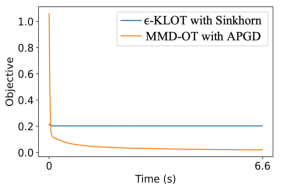
\includegraphics[width=0.47\linewidth]{chapter-1/images/synth3.pdf}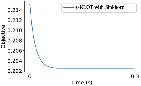
\includegraphics[width=0.5\linewidth]{chapter-1/images/time.pdf}
    \caption{Computation time: Convergence plots with $m=5000$ for the case of the same source and target measures where the optimal objective is expected to be 0. Left: MMD-OT Problem (\ref{eqn:kernot}) solved with accelerated projected gradient descent. Right: $\epsilon$-KLOT's convergence plot is shown separately. We observe that $\epsilon$-KLOT's objective plateaus in 0.3 seconds. We note that our convergence to the optimal objective is faster than that of $\epsilon$-KLOT.}
    \label{time-supp}
\end{figure}
\paragraph{Sample Complexity.}
\begin{figure}[t]
    \centering
    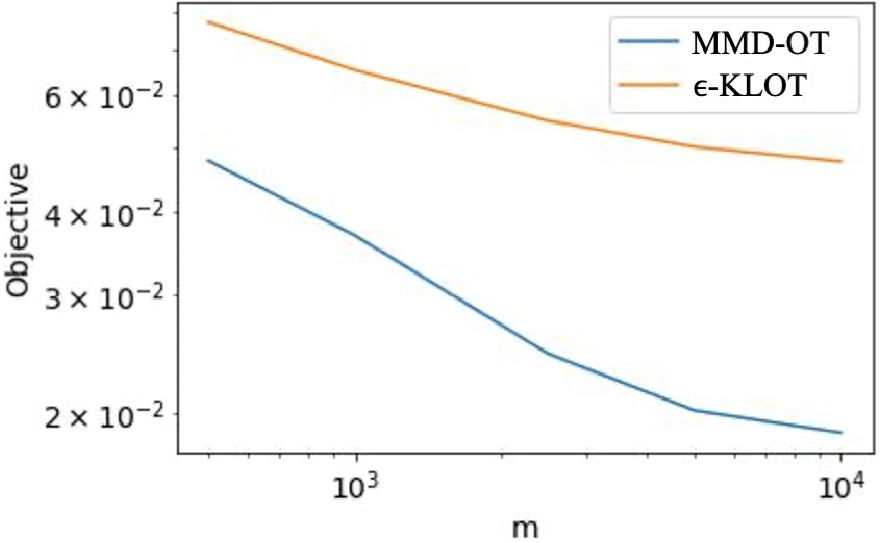
\includegraphics[scale=0.5]{chapter-1/images/sc.pdf}
    \caption{Sample efficiency: Log-log plot of optimal objective vs number of samples. The optimal objective values of MMD-OT and $\epsilon$-KLOT formulation are shown as the number of samples increases. The data lies in 10 dimensions, and the source and target measures are both Uniform. MMD-OT can be seen to have a better rate of convergence.}
    \label{samp-supp}
\end{figure}
In Theorem~\ref{thm:cons}, we proved an attractive sample complexity of $O\left(m^{-\frac{1}{2}}\right)$ for our sample-based estimators. In this section, we present a synthetic experiment to show that the convergence of MMD-OT's metric towards the true value is faster than that of $\epsilon$-KLOT. We sample 10-dimensional sources and target samples from Uniform sources and target marginals, respectively. As the marginals are equal, the metrics over measures should converge to 0 as the number of samples increases. We repeat the experiment with an increasing number of samples. 
% In our experimental setup, we follow conditions given in~\citep{Liero2018} so that $\epsilon$-KLOT gives a metric. 
We use squared-Euclidean cost. For $\epsilon$-KLOT, $\lambda=1, \epsilon=1e-2$. For MMD-OT, $\lambda=1$ and RBF kernel with $\sigma=1$ is used. In Figure~\ref{samp-supp}, we plot MMD-OT's objective and the square root of the $\epsilon$-KLOT objective on increasing the number of samples. It can be seen from the plot that the MMD-OT achieves a better rate of convergence compared to $\epsilon$-KLOT.
\paragraph{Effect of Regularization.} In Figures~\ref{fig:reg-bal} and~\ref{fig:reg-unb}, we visualize matching the marginals of MMD-OT's optimal transport plan. We show the results with both RBF kernel $k(x, y) = \exp{\left(\frac{-\|x-y\|^2}{2*10^{-6}}\right)}$ and the IMQ kernel $k(x, y) = \left(10^{-6}+\|x-y\|^2\right)^{-0.5}$. As we increase $\lambda$, the matching becomes better for unnormalized measures, and the marginals exactly match the given measures when the measures are normalized. We have also shown the unbalanced case results with $\epsilon$-KLOT. As the POT library~\citep{flamary2021pot} doesn't allow including a simplex constraint for $\epsilon$-KLOT, we do not show this.
\begin{figure*}[t]
    \centering
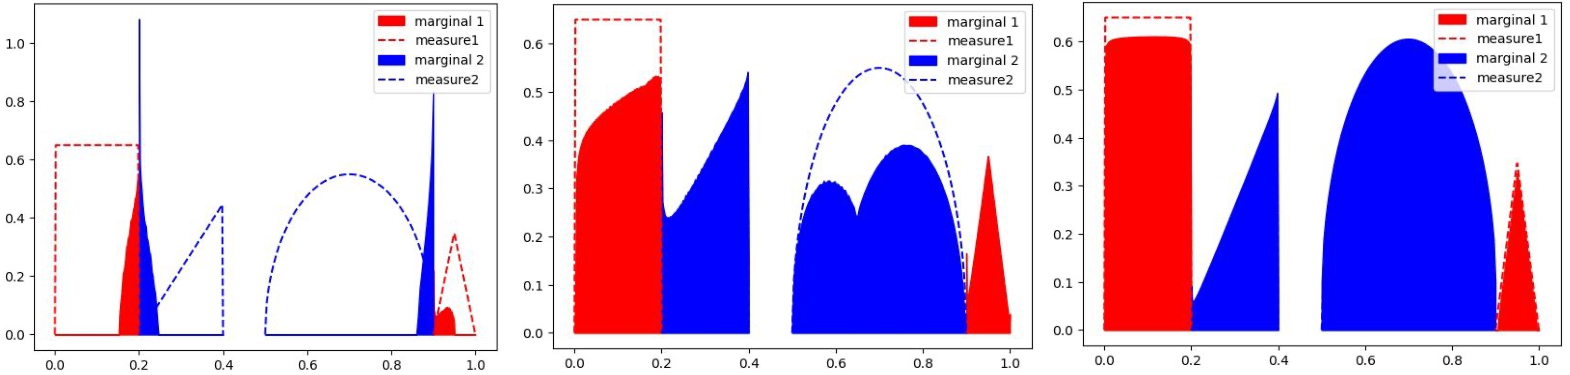
\includegraphics[width=\linewidth]{chapter-1/images/unb-IMQ.pdf}\\
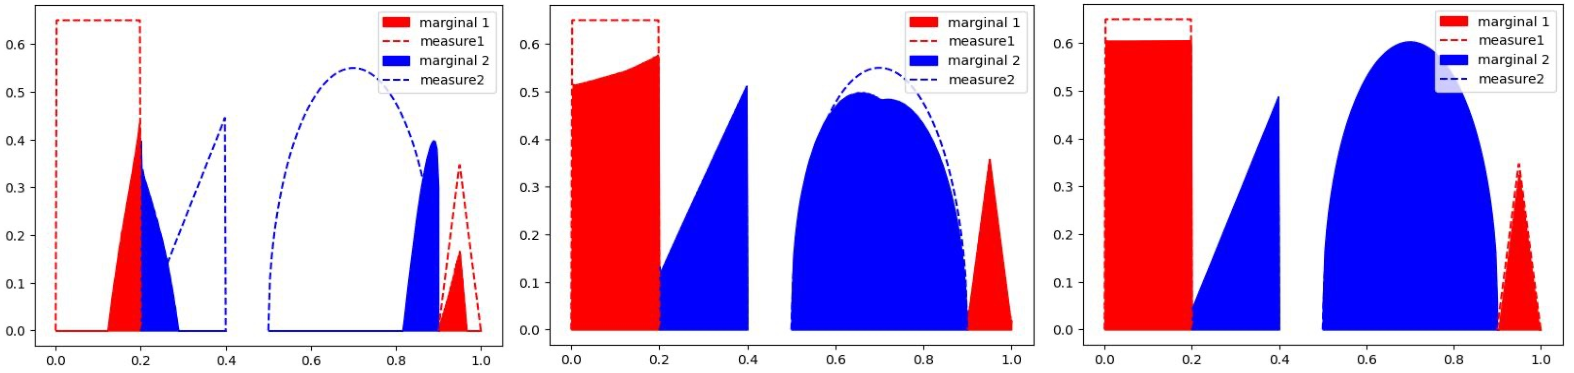
\includegraphics[width=\linewidth]{chapter-1/images/unb-RBF.pdf}\\
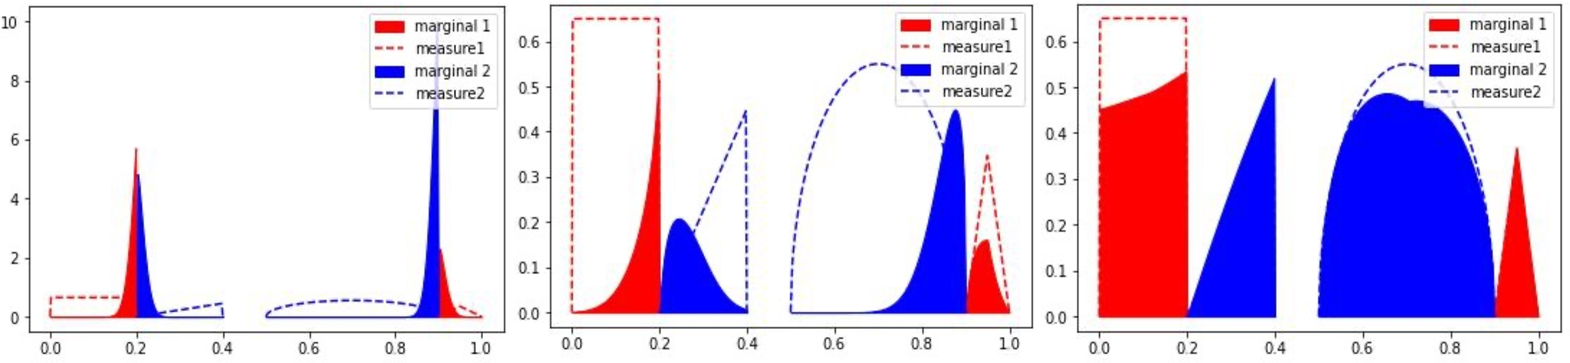
\includegraphics[width=\linewidth]{chapter-1/images/unb-KL.pdf}
    \caption{(With unnormalized measures) Visualizing the marginals of transport plans learnt by MMD-OT (row 1 with IMQ kernel, row 2 with RBF kernel) and $\epsilon$-KLOT (row 3), on increasing the regularization hyperparameter $\lambda$.}
    \label{fig:reg-unb}
\end{figure*}

\begin{figure*}[t]
    \centering
    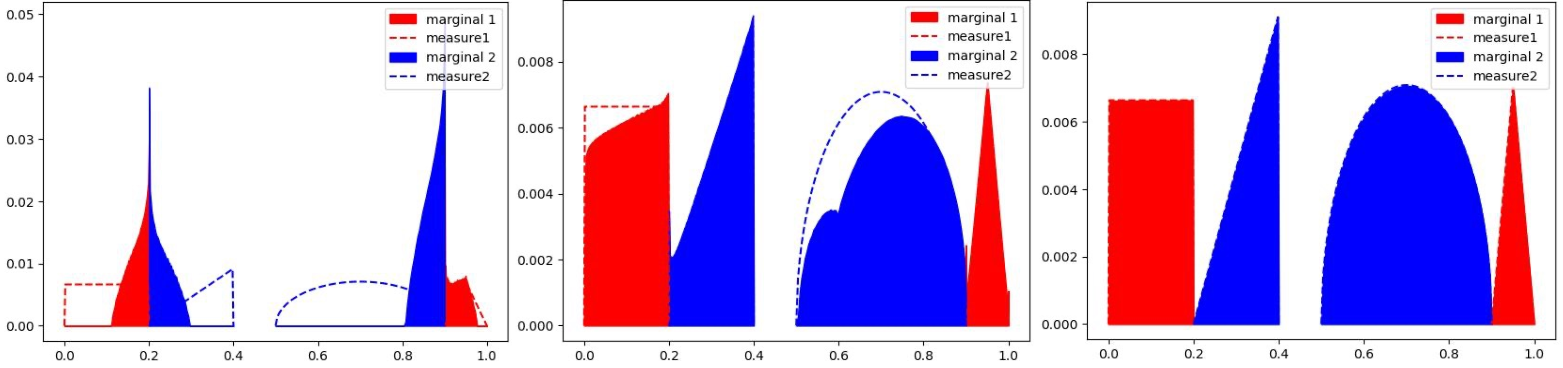
\includegraphics[width=\linewidth]{chapter-1/images/bal-IMQ.pdf}\\
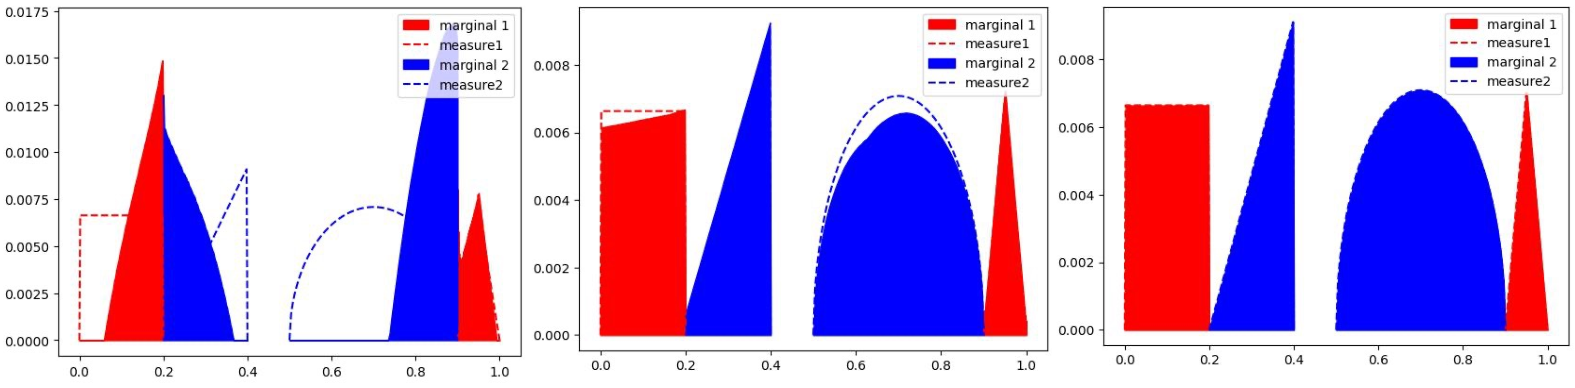
\includegraphics[width=\linewidth]{chapter-1/images/bal-RBF.pdf}
    \caption{(With normalized measures) Visualizing the marginals of MMD-OT (row 1 with IMQ kernel, row 2 with RBF kernel), solved with simplex constraints, plan on increasing the regularization hyperparameter $\lambda$. We do not show $\epsilon$-KLOT here as the Sinkhorn algorithm for solving $\epsilon$-KLOT in the POT library~\citep{flamary2021pot} does not incorporate the Simplex constraints on the transport plan.}
    \label{fig:reg-bal}
\end{figure*}

\subsection{Two-sample Test}\label{app:tst}
Following~\cite{dktst}, we repeat the experiment 10 times, and in each trial, we randomly sample a validation subset and a test subset of size $N$ from the given real and fake MNIST datasets. We run the two-sample test experiment for Type-II error on the test set for a given trial using the hyperparameters chosen for that trial. The hyperparameters were tuned for $m=100$ for each trial. The hyperparameters for a given trial were chosen based on the average empirical test power (higher is better) over that trial's validation dataset. 

We use squared-Euclidean distance for MMD-OT and $\epsilon$-KLOT formulations. RBF kernel, $k(x, y) = \exp{\left(\frac{-\|x-y\|^2}{2\sigma^2}\right)}$, is used for MMD and for MMD-OT formulation. The hyperparameters are chosen from the following set. For the MMD-OT and MMD, $\sigma$ was chosen from \{\textup{median}, 40, 60, 80, 100\} where the median is the median-heuristic~\citep{gretton12a}. For the MMD-OT an $\epsilon$-KLOT, $\lambda$ is chosen from \{0.1, 1, 10\}. For $\epsilon$-KLOT, $\epsilon$ was chosen from \{1, $10^{-1}, 10^{-2}, 10^{-3}, 10^{-4}$\}. Based on validation, $\sigma$ as the median is chosen for MMD at all trials. For $\epsilon$-KLOT, the best hyperparameters $(\lambda, \epsilon)$ are (10, 0.001) for trial number 3, (0.1, 0.1) for trial number 10 and (1, 0.1) for the remaining the 8 trials. For MMD-OT, the best hyperparameters $(\lambda, \sigma^2)$ are $(0.1, 60)$ for trial number 9 and $(1, \textup{median}^2)$ for the remaining 9 trials.

\paragraph{Additional Results.}
Following \cite{dktst}, we consider the task of verifying that the datasets CIFAR-10~\citep{Krizhevsky2009LearningML} and CIFAR-10.1~\citep{Recht2018DoCC} are statistically different. We follow the same experimental setup as given in~\cite{dktst}. The training is done on 1000 images from each dataset, and the test is on 1031 images. The experiment is repeated 10 times, and the average test power is compared with the results shown in~\cite{dktst} with the popular baselines: ME~\citep{ME, ME2}, SCF~\citep{ME, ME2}, C2ST-S~\citep{C2STS-S}, C2ST-L~\citep{C2ST-L}. We repeat the experiment following the same setup for the MMD and $\epsilon$-KLOT baselines. The chosen hyperparameters $(\lambda, \epsilon)$ for the 10 different experimental runs $\epsilon$-KLOT are: 
\newline $(0.1, 0.1), (1, 0.1), (1, 0.1), (1, 0.01), (1, 0.1), (1, 0.1), (1, 0.1), (0.1, 0.1), (1, 0.1), (1, 0.1)$ and $(1, 0.1)$. 
The chosen $(\lambda, \sigma^2)$ for the 10 different experimental runs of MMD-OT are: \newline$(0.1, \textup{median}), (1, 60), (10, 100), (0.1, 80), (0.1, 40), (0.1, 40), (0.1, 40), (1, \textup{median}), (0.1, 80)$ and $(1, 40)$.
Table~\ref{2st-cifar} shows that the proposed MMD-OT obtains the highest test power.

\begin{table}[t]
\caption{Test power (higher is better) for the task of CIFAR-10.1 vs CIFAR 10. The proposed MMD-OT method achieves the best results.}
\label{2st-cifar}
\centering
\begin{tabular}{ccccccc}
%\hline
\toprule
ME & SCF & C2ST-S & C2ST-L & MMD & $\epsilon$-KLOT & \cellcolor{green!10}{Proposed (MMD-OT)}\\
\midrule
0.588 & 0.171 & 0.452 & 0.529 & 0.316 & 0.132 & \cellcolor{green!10}{\textbf{0.643}}\\
\bottomrule
\end{tabular}
% \end{center}
\end{table}

\subsection{Single-Cell RNA sequencing}\label{appendix:scrna}
scRNA-seq helps us understand how the expression profile of the cells changes over stages~\citep{bioapp19}. 
A population of cells is represented as a measure of the gene expression space, and as they grow/divide/die, and the measure evolves over time. 
While scRNA-seq records such a measure at a time stamp, it does so by destroying the cells~\citep{bioapp19}. Thus, it is impossible to monitor how the cell population evolves continuously over time. In fact, only a few measurements at discrete timesteps are generally taken due to the cost involved. 

We perform experiments on the Embryoid Body (EB) single-cell dataset~\citep{moon19a}. The Embryoid Body dataset comprises data at 5 timesteps with sample sizes as 2381, 4163, 3278, 3665 and 3332, respectively.

The MMD barycenter interpolating between measures $s_0, t_0$ has the closed form solution as $\frac{1}{2}(s_0+t_0)$. For evaluating the performance at timestep $t_i$, we select the hyperparameters based on the task of predicting for $\{t_1, t_2, t_3\}\setminus \{t_i\}$. We use IMQ kernel $k(x, y) = \left(\frac{1+\|x-y\|^2}{\sigma^2}\right)^{-0.5}$. The $\lambda$ hyperparameter for the validation of MMD-OT is chosen from $\{0.1, 1, 10\}$ and $\sigma^2$ is chosen from $\{1e-4, 1e-3, 1e-2, 1e-1, \textup{median}\}$, where median denotes the median of \{$0.5\|x-y\|^2\ \forall x, y\in\mathcal{D} \textup{ s.t. } x\neq y$\} over the training minibatch ($\mathcal{D}$). The chosen $(\lambda, \sigma^2)$ for timesteps $t_1, t_2, t_3$ are (1, 0.1), (1, median) and (1, median), respectively. The $\lambda$ hyperparameter for the validation of $\epsilon$-KLOT is chosen from $\{0.1, 1, 10\}$ and $\epsilon$ is chosen from $\{1e-5, 1e-4, 1e-3, 1e-2, 1e-1\}$. The chosen $(\lambda, \epsilon)$ for timesteps $t_1, t_2, t_3$ are (10, 0.01), (1, 0.1) and (1, 0.1) respectively. In Table~\ref{app:2st-mnist-2}, we compare against additional OT-based methods $\bar{W}_{c,1}, \bar{W}_{c,2}, \epsilon$-OT.
\begin{table}[t]
\caption{Additional OT-based baselines for two-sample test: Average Test Power (between 0 and 1; higher is better) on MNIST. MMD-OT obtains the highest average test power at all timesteps, even with the additional baselines. The significance level is 0.05.}
\label{app:2st-mnist-2}
\centering
% \begin{center}
\begin{tabular}{ccccccc}
%\hline
\toprule
$m$ & $\bar{W}_{c,1}$ & $\bar{W}_{c,2}$ & $\epsilon$-OT & \cellcolor{green!10}{Proposed (MMD-OT)} \\
\midrule
%\hline
100 & 0.111 & 0.099 & 0.108 & \cellcolor{green!10}{\textbf{0.154}}\\
200 & 0.232 & 0.207 & 0.191 & \cellcolor{green!10}{\textbf{0.333}}\\
300 & 0.339 & 0.309 & 0.244 & \cellcolor{green!10}{\textbf{0.588}}\\
400 & 0.482 & 0.452 & 0.318 & \cellcolor{green!10}{\textbf{0.762}}\\
500 & 0.596 & 0.557 & 0.356 & \cellcolor{green!10}{\textbf{0.873}}\\ 
1000 & 0.805 & 0.773 & 0.508 & \cellcolor{green!10}{\textbf{0.909}}\\ 
%\hline
\bottomrule
\end{tabular}
% \end{center}
\end{table}


\begin{figure}[t]
\centering
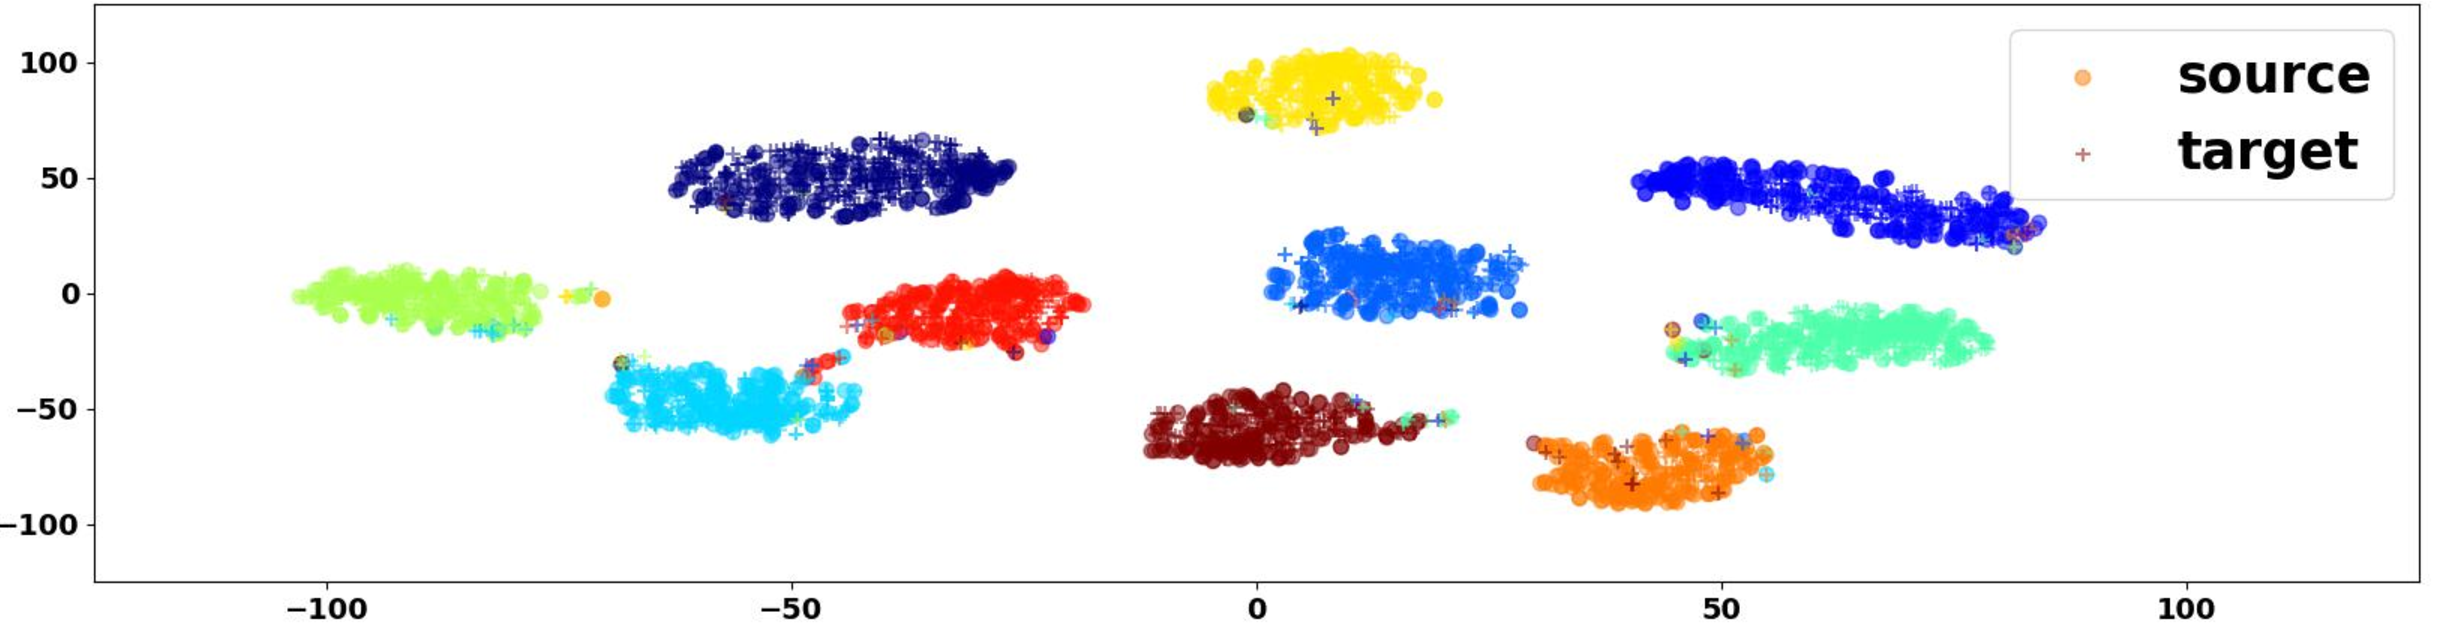
\includegraphics[width=0.6\linewidth]{chapter-1/images/KL-tsne.pdf}\\
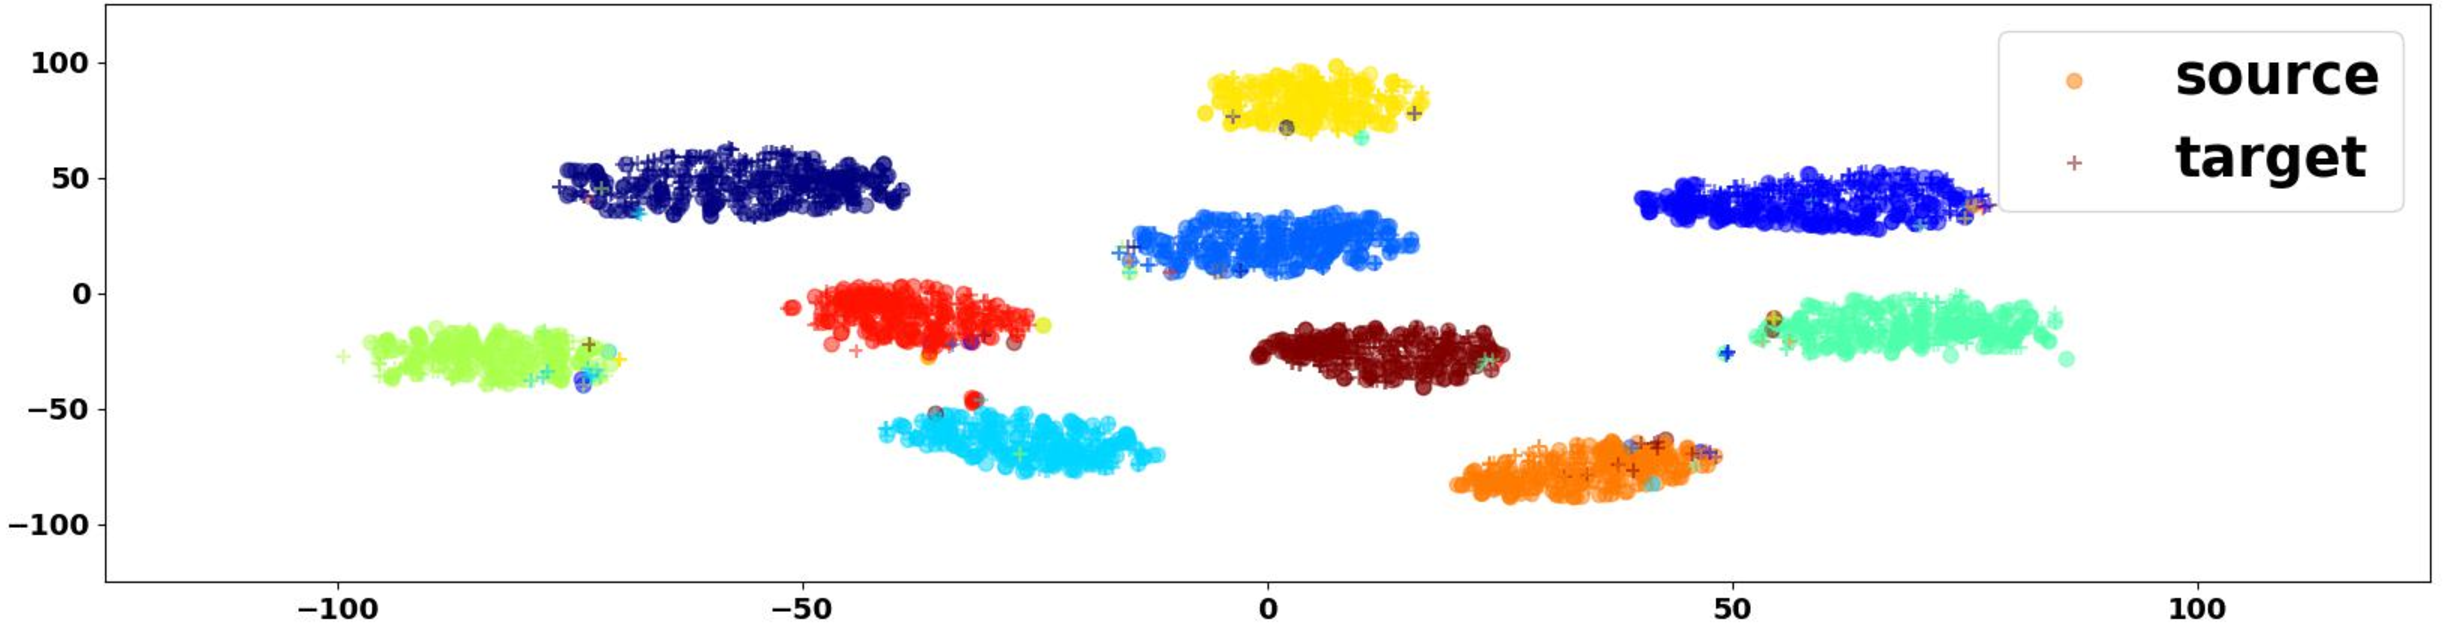
\includegraphics[width=0.6\linewidth]{chapter-1/images/MMDOT-tsne.pdf}
\caption{(Best viewed in color) The t-SNE plots of the source and target embeddings learnt for the M-MNIST to USPS domain adaptation task with $\epsilon$-KLOT (row 1) and MMD-OT (row 2). Different cluster colors imply different classes. The quality of the learnt representations can be judged based on the separation between clusters. The clusters obtained by MMD-OT seem better separated (for example, the red and the cyan-colored clusters).}
\label{tsne}
\end{figure}

\subsection{Domain Adaptation in JUMBOT framework}\label{app:jumbot} The experiments are performed with the same seed as used by JUMBOT. For the experiment on the Digits dataset, the chosen hyperparameters for MMD-OT are $\sigma^2$ in the IMQ kernel $k(x, y) = \left(\frac{1+\|x-y\|^2}{\sigma^2}\right)^{-0.5}$ as $10^{-2}$ and $\lambda$ as 100. In Figure~\ref{tsne}, we also compare the t-SNE plot of the embeddings learnt with the MMD-OT and $\epsilon$-KLOT-based loss. The clusters formed with the proposed MMD-OT seem better separated (for example, the red and the cyan-colored clusters).
For the experiment on the Office-Home dataset, the chosen hyperparameters for MMD-OT are \Big($\lambda=100$, IMQ kernel with $\sigma^2=0.1$\Big). For the VisDA-2017 dataset, the chosen hyperparameters for MMD-OT are \Big($\lambda=1$, IMQ kernel with $\sigma^2$ as 10\Big).

For the validation phase on the Digits and the Office-Home datasets, we choose $\lambda$ from the set $\{1, 10, 100\}$ and $\sigma^2$ from the set $\{0.01, 0.1, 10, 100, \textup{median}\}$. For the validation phase on VisDA, we choose $\lambda$ from the set $\{1, 10, 100\}$ and $\sigma^2$ from the set $\{0.1, 10, 100\}$. 

% \begin{figure}[t]
%     \centering  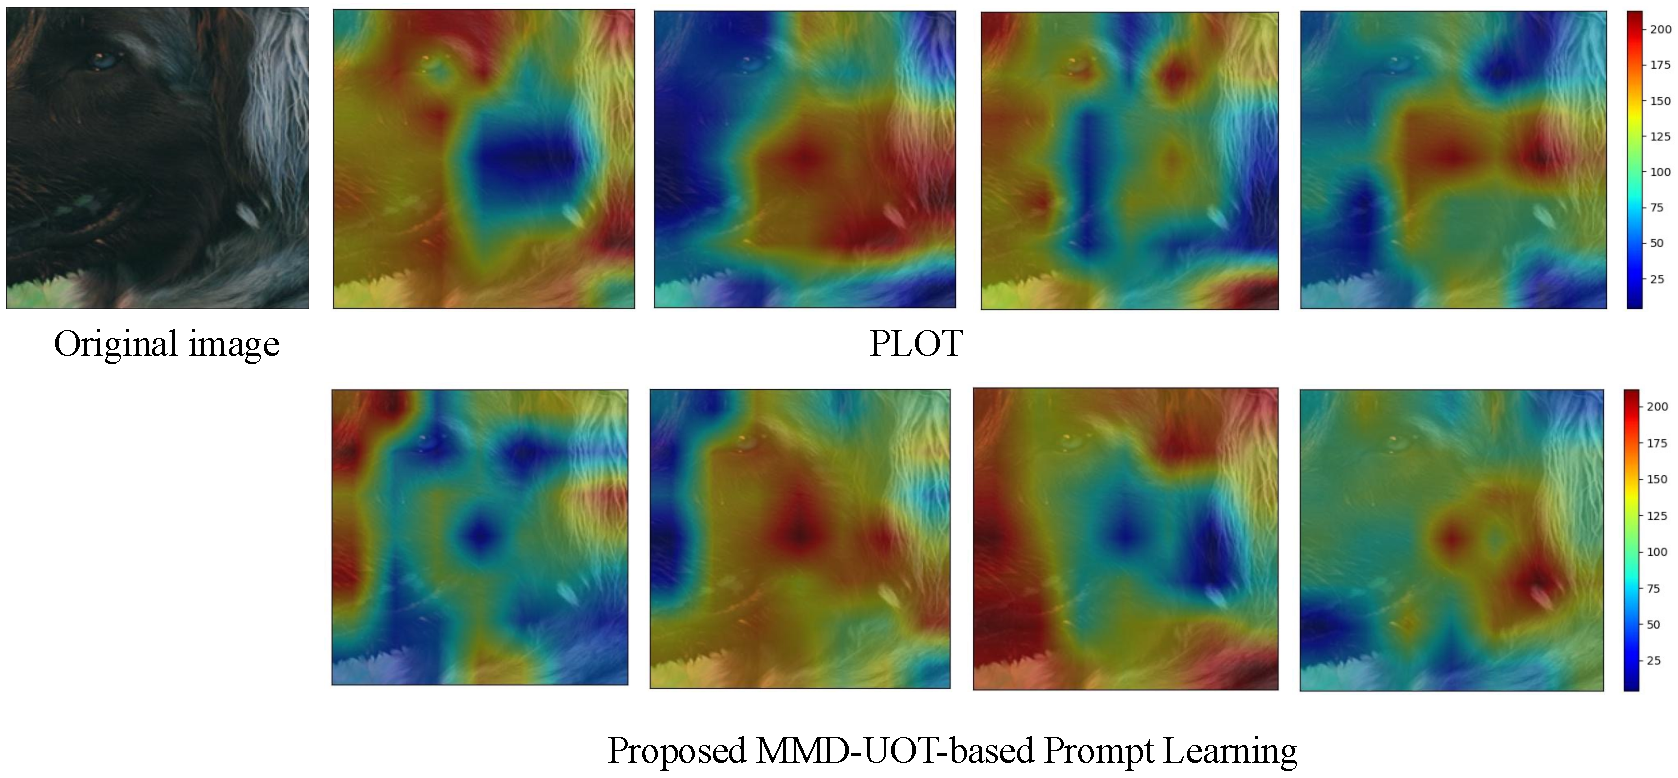
\includegraphics[scale=0.5]{chapter-1/images/plot-viz-dog.pdf}
%     \caption{The attention maps corresponding to each of the 4 prompts for the baseline (PLOT) and the proposed method. The prompts learnt using the proposed MMD-OT capture diverse attributes for identifying the dog (Oxford-Pets dataset): the forehead and the nose, the right portion of the face, the head along with the left portion of the face, and the ear.
%     }
%     \label{fig:prompt-dog}
% \end{figure}

\begin{table*}[ht!]
    \caption{Hyperparameters (kernel type, kernel hyperparameter, $\lambda$) for the prompt learning experiment.}\label{prompthp}
    \centering
    % \begin{center}
    \footnotesize{
    \begin{tabular}{lccccc}
    \toprule
       Dataset & 1 & 2 & 4 & 8 & 16\\
       \toprule
        EuroSAT  & (imq2, $10^{-3}, 500$) & (imq1, $10^4, 10^3$) & (imq1, $10^{-2}$, 500) & (imq1, $10^4, 500$) & (rbf, 1, 500) \\
        DTD  & (imq1, $10^{-2}$, 10) & (rbf, 100, 100) & (imq2, $10^{-2}$, 10) & (rbf, $10^{-2}, 10$) & (rbf, 0.1, 1)\\
        Oxford-Pets  & (imq2, 0.01, 500) & (rbf, $10^{-3}, 10$) & (imq, 1, 10) & (imq1, 0.1, 10)  & (imq1, 0.01, 1)\\
        UCF101 & (rbf, 1, 100) & (imq2, 10, 100) & (rbf, 0.01, 1000) & (rbf, $10^{-4}$, 10) & (rbf, 100, $10^3$)\\
        \bottomrule
    \end{tabular}}
    % \end{center}
\end{table*}
\begin{figure}[t]
    \centering
    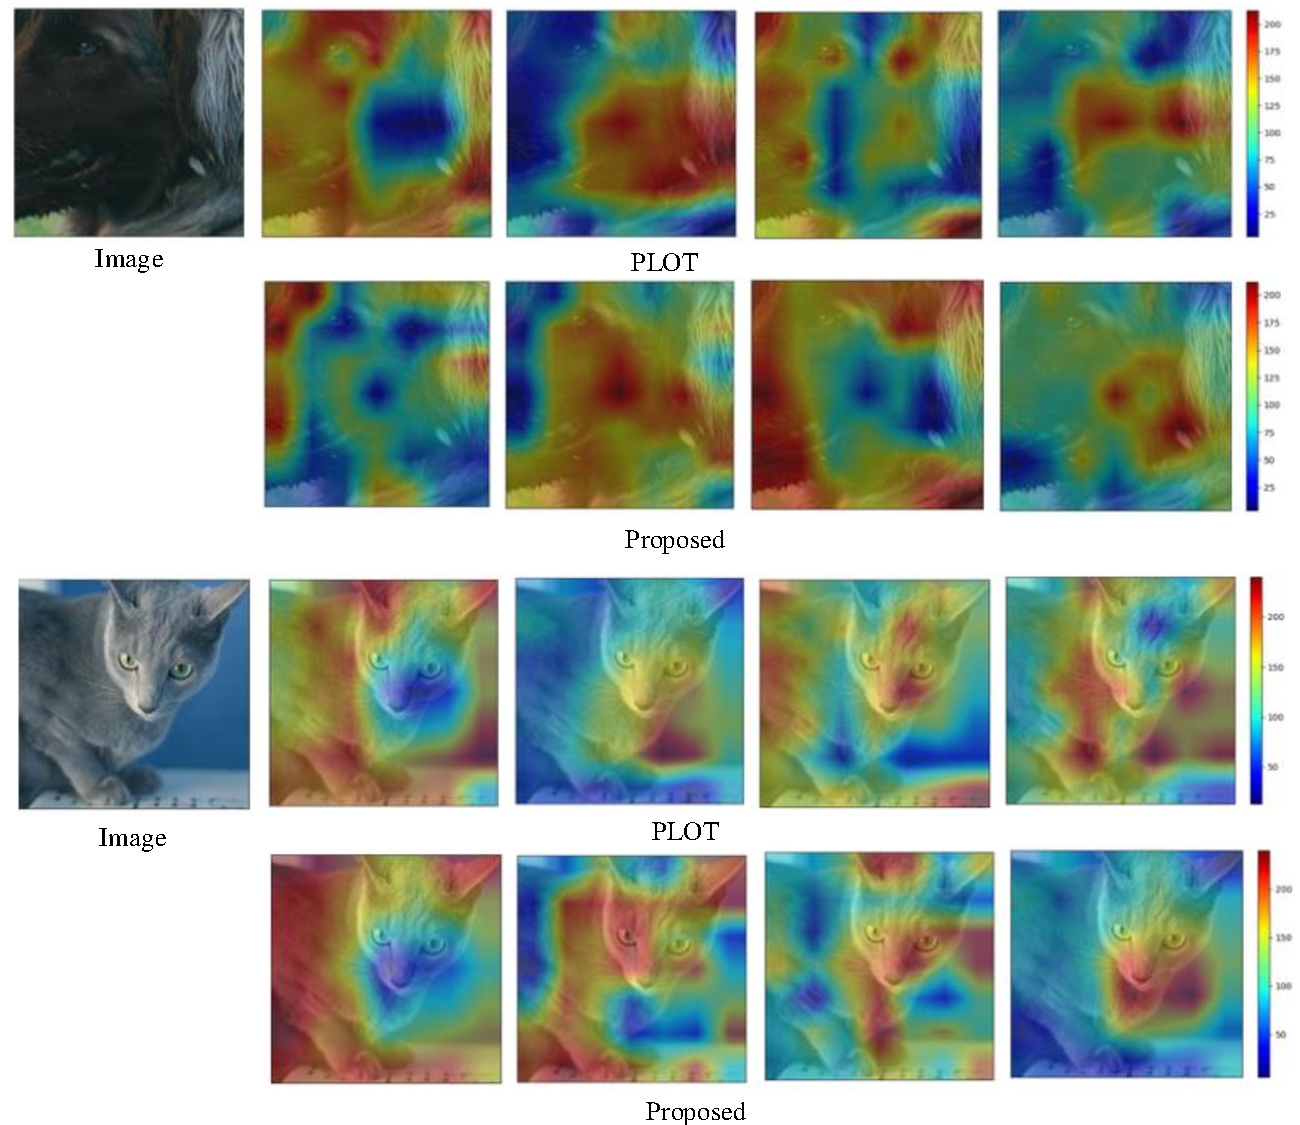
\includegraphics[scale=0.5]{chapter-1/images/PLOT-APP.pdf}   
    \caption{The attention maps corresponding to each of the four prompts for the baseline (PLOT) and the proposed method. The prompts learnt using the proposed MMD-OT capture diverse attributes for identifying the cat (Oxford-Pets dataset): lower body, upper body, image background and the area near the mouth. Similarly, the prompts learnt using the proposed MMD-OT capture diverse attributes for identifying the dog (Oxford-Pets dataset): the forehead and the nose, the right portion of the face, the head along with the left portion of the face, and the ear.
    }
    \label{fig:prompt-cat}
\end{figure}
\subsection{Prompt Learning}\label{app:prompt}
Let $\mathbf{F}=\{\mathbf{f}_m|_{m=1}^M\}$ denote the set of visual features for a given image and $\mathbf{G}'_r=\{\mathbf{g}_n|_{n=1}^N\}$ denote the set of textual prompt features for class $r$. Following the setup in the PLOT baseline, an OT distance is computed between empirical measures over 49 image features and 4 textual prompt features, taking cosine similarity cost. Let $d_{OT}(\mathbf{x}, r)$ denote the OT distance between the visual features of image $\mathbf{x}$ and prompt features of class $r$. The prediction probability is given by
$
    p(y=r|\mathbf{x}) = \frac{\exp{\left((1-d_{OT}(\mathbf{x}, r)/\tau)\right)}}{\sum_{r=1}^T\exp{\left((1-d_{OT}(\mathbf{x}, r)/\tau)\right)}},
$ where $T$ denotes the total no. of classes and $\tau$ is the temperature of softmax. The textual prompt embeddings are then optimized with the cross-entropy loss. Additional results on Oxford-Pets~\citep{oxp} and UCF101~\citep{DBLP:journals/corr/abs-1212-0402} datasets are shown in Table~\ref{app:tableplot}. The attention maps corresponding to the prompts learnt are shown in Fig.~\ref{fig:prompt-cat} which exhibit the desired diversity.

Following the PLOT baseline, we use the last-epoch model. The authors empirically found that learning 4 prompts with the PLOT method gave the best results. In our experiments, we keep the number of prompts and the other neural network hyperparameters fixed. We only choose $\lambda$ and the kernel hyperparameters for prompt learning using MMD-OT. For this experiment, we also validate the kernel type. Besides RBF, we consider two kernels belonging to the IMQ family: $k(x, y) = \left(\frac{1+\|x-y\|^2}{\sigma^2}\right)^{-0.5}$ (referred to as imq1) and $k(x, y) = (\sigma^2+\|x-y\|^2)^{-0.5}$ (referred to as imq2). We choose $\lambda$ from \{10, 100, 500, 1000\} and kernel hyperparameter ($\sigma^2$) from \{$1e-3, 1e-2, 1e-1, 1, 10, 1e+2, 1e+3$\}. The chosen hyperparameters are included in Table~\ref{prompthp}.

\begin{table*}[t]
\caption{Additional Prompt Learning results. Average and standard deviation (over 3 runs) of accuracy (higher is better) on the $\mathcal{F}$-shot classification task, shown for different values of shots ($\mathcal{F}$) in the state-of-the-art PLOT framework. The proposed method replaces OT with MMD-OT in PLOT, keeping all other hyperparameters the same. The results of PLOT are taken from their paper~\citep{chen2023plot}.} \label{app:tableplot} 
\centering
\footnotesize{
\begin{tabular}{llccccc}
\toprule
Dataset & Method & 1 & 2 & 4 & 8 & 16 \\
\midrule
\multirow{ 2}{*}{EuroSAT} & PLOT & 54.05 $\pm$ 5.95 & 64.21 $\pm$ 1.90 & \textbf{72.36} $\pm$ \textbf{2.29} & 78.15 $\pm$ 2.65 & 82.23 $\pm$ 0.91 \\ 
 & \cellcolor{green!10}{Proposed} & \cellcolor{green!10}{\textbf{58.47} $\pm$ \textbf{1.37}} & \cellcolor{green!10}{\textbf{66.0} $\pm$ \textbf{0.93}} & \cellcolor{green!10}{71.97 $\pm$ 2.21} & \cellcolor{green!10}{\textbf{79.03} $\pm$ \textbf{1.91}} & \cellcolor{green!10}{\textbf{83.23} $\pm$ \textbf{0.24}}\\ 
\midrule
\multirow{ 2}{*}{DTD} & PLOT & 46.55 $\pm$ 2.62 & \textbf{51.24} $\pm$ \textbf{1.95} & 56.03 $\pm$ 0.43  & 61.70 $\pm$ 0.35 & 65.60 $\pm$ 0.82\\ 
 & \cellcolor{green!10}{Proposed} & \cellcolor{green!10}{\textbf{47.27}$\pm$\textbf{1.46}} & \cellcolor{green!10}{51.0$\pm$1.71} & \cellcolor{green!10}{\textbf{56.40}$\pm$\textbf{0.73}} & \cellcolor{green!10}{\textbf{63.17}$\pm$\textbf{0.69}} & \cellcolor{green!10}{\textbf{65.90} $\pm$ \textbf{0.29}}\\ 
 \bottomrule
 \multirow{ 2}{*}{Oxford-Pets} & PLOT & 87.49 $\pm$ 0.57 & 86.64  $\pm$ 0.63 & 88.63 $\pm$ 0.26 & \textbf{87.39} $\pm$ \textbf{0.74} & 87.21  $\pm$ 0.40\\ 
 & \cellcolor{green!10}{Proposed} & \cellcolor{green!10}{\textbf{87.60} $\pm$ \textbf{0.65}} & \cellcolor{green!10}{\textbf{87.47} $\pm$ \textbf{1.04}} & \cellcolor{green!10}{\textbf{88.77} $\pm$ \textbf{0.46}} & \cellcolor{green!10}{87.23 $\pm$ 0.34} &  \cellcolor{green!10}{\textbf{88.27} $\pm$ \textbf{0.29}} \\  
 \midrule
 \multirow{ 2}{*}{UCF101} & PLOT & \textbf{64.53} $\pm$ \textbf{0.70} & 66.83 $\pm$ 0.43 & 69.60  $\pm$ 0.67 & 74.45 $\pm$ 0.50 & 77.26 $\pm$ 0.64 \\ 
 & \cellcolor{green!10}{Proposed} & \cellcolor{green!10}{64.2 $\pm$ 0.73} & \cellcolor{green!10}{\textbf{67.47} $\pm$ \textbf{0.82}} & \cellcolor{green!10}{\textbf{70.87} $\pm$ \textbf{0.48}} & \cellcolor{green!10}{\textbf{74.87} $\pm$ \textbf{0.33}} & \cellcolor{green!10}{\textbf{77.27} $\pm$ \textbf{0.26}}  \\
 \midrule
\multirow{ 2}{*}{\textbf{Avg.}} & PLOT & 63.16 & 67.23 & 71.66 & 75.42 & 78.08 \\ 
 & \cellcolor{green!10}{Proposed} & \cellcolor{green!10}{\textbf{64.38}} & \cellcolor{green!10}{\textbf{67.98}} & \cellcolor{green!10}{\textbf{72.00}} & \cellcolor{green!10}{\textbf{76.08}} & \cellcolor{green!10}{\textbf{78.67}}\\
 \bottomrule
\end{tabular}}
% \end{center}

\end{table*}


%%
\resumetoc